% Cal Poly Thesis
% based on UC Thesis format
% modified by Mark Barry 2/07.
\documentclass[12pt]{ucthesis}

% Different font in captions (single-spaced, bold) ------------
\newcommand{\captionfonts}{\small\bf\ssp}

\makeatletter  % Allow the use of @ in command names
\long\def\@makecaption#1#2{%
  \vskip\abovecaptionskip
  \sbox\@tempboxa{{\captionfonts #1: #2}}%
  \ifdim \wd\@tempboxa >\hsize
    {\captionfonts #1: #2\par}
  \else
    \hbox to\hsize{\hfil\box\@tempboxa\hfil}%
  \fi
  \vskip\belowcaptionskip}
\makeatother   % Cancel the effect of \makeatletter
% ---------------------------------------

%formatting/structure based packages
   \usepackage[letterpaper]{geometry}
   \usepackage[overload]{textcase}

%packages necessary for content
   \usepackage{url}
   \usepackage{graphicx}
   \usepackage{amssymb}
   \usepackage{amsmath}
   \usepackage{mathtools}
   \usepackage{dsfont}
   \usepackage{algorithmicx}
   \usepackage{algpseudocode}
   \usepackage{multirow}
   \usepackage{subcaption}

   \usepackage[utf8]{inputenc}
   \usepackage[russian,english]{babel}

%paper formatting
   \setlength{\parindent}{0.25in} \setlength{\parskip}{6pt}
   \geometry{verbose,nohead,tmargin=1.25in,bmargin=1in,lmargin=1.5in,rmargin=1.3in}
   \setcounter{tocdepth}{2}

\begin{document}

% Declarations for Front Matter
\title{Algorithms for Library-based Microbial Source Tracking}
\author{Aldrin Montana}
\degreemonth{June}
\degreeyear{2013}
\degree{Master of Science}
\field{Computer Science}
\campus{San Luis Obispo}

\defensemonth{June}
\defenseyear{2013}

\numberofmembers{4}
   \chair{Alexander Dekhtyar, Ph.D.}
   \othermemberA{Chris Lupo, Ph.D.}
   \othermemberB{Tim Kearns, Ph.D.}
   \othermemberC{Michael Black, Ph.D.}
   %\othermemberD{Eriq Augustine, M.S.}
\copyrightyears{seven}

\maketitle
\begin{frontmatter}
   % Custom made for Cal Poly (by Mark Barry, modified by Andrew Tsui).
   \copyrightpage

   % Custom made for Cal Poly (by Andrew Tsui).
   \committeemembershippage

   \begin{abstract}
      Pyroprinting is a novel, library-based microbial source tracking method
      developed by the biology department at Cal Poly, San Luis Obispo. This
      method consists of two parts: (1) sample collection and pyroprinting (2)
      comparison of produced pyroprints against a database. Cal Poly Library of
      Pyroprints (CPLOP) is a web-based database application that provides
      storage and analysis of pyroprints. CPLOP currently contains 10000
      pyroprints and is growing rapidly as students and researchers continue
      adding data. The traditional method of analysis used by biologists,
      \textsf{agglomerative hierarchical clustering}, is inadequate. While the
      clusters it produces are acceptable, pyroprinting requires a method of
      analysis that is both scalable and flexible. \textsf{Agglomerative
      hierarchical clustering} falls short in these regards as it is unable to
      efficiently incorporate incremental updates and is incapable of utilizing
      available meta-data. We propose \textsf{ontology-based hierarchical
      clustering} (\textsf{OHClust!}), a modification of \textsf{agglomerative
      hierarchical clustering} that expresses meta-data-based relationships as
      an ontology to direct the order in which hierarchical clustering
      algorithms analyze the data. In this thesis, the strengths and weaknesses
      of \textsf{OHClust!} are discussed, and its performance is analyzed in
      comparison to \textsf{agglomerative hierarchical clustering}.
   \end{abstract}

   \begin{acknowledgements}
      This work was supported in part by grants from:
      \begin{itemize}
         \item The W.M. Keck Foundation
         \item The National Science Foundation
      \end{itemize}
      I would like to specially thank the following for making my time at Cal
      Poly a great and memorable adventure:
      \begin{itemize}
         \item The department staff, especially Christy Zolla, known both as
               \textit{the goddess of wisdom and light} and my CSC mom, for
               making the bureaucratic process a cynch.
         \item My family and friends, particularly my mom, step dad,
               and dad, for all that they've done to support me.
         \item The great and wonderful biologists, Jen VanderKelen and Emily
               Neal, for being awesome and patient in working with me.
         \item Chris Kitts and Michael Black for being fun and enjoyable to
               work with. It's the peanut gallery and poop jokes that make
               working with biologists a particularly good time.
         \item Anya Goodman for being the first to work with me, and for still
               being willing to work with me after three years. Special thanks
               for being really great and always making me sound and feel like
               an amazing person/wizard.
         \item Alex Dekhtyar for being the best adviser I could have asked for.
               I believe all of my growth can be attributed to the guidance
               that Alex has provided me. I cannot thank you enough for the
               great wisdom, knowledge, and time that I've had at Cal Poly for
               the last three years.
         \item \foreignlanguage{russian}{квас} for always being there to soothe
               the soul.
         \item My roommates who have always provided me with a family away from
               home. Our unity is strong.
      \end{itemize}
   \end{acknowledgements}

   \tableofcontents

   \listoftables
   \listoffigures
\end{frontmatter}

\pagestyle{plain}

\renewcommand{\baselinestretch}{1.66}

%%%%%%%%%%%%%%%%%%%%%%%%%%%%%%%%%%%%%%%%%%%%%%%%%%%%%%%%%%%%%%%%%%%%%%%%%%%%%%%
%%%%%%%%%%%%%% ----------------- Main chapters ---------------------- %%%%%%%%%
%%%%%%%%%%%%%%%%%%%%%%%%%%%%%%%%%%%%%%%%%%%%%%%%%%%%%%%%%%%%%%%%%%%%%%%%%%%%%%%

\chapter{Introduction}\label{chap:intro}
   To maintain the cleanliness of current ``fishable and swimmable'' bodies of
   water, and improve the cleanliness of other bodies of water, health and
   environmental protection agencies have been interested in the ability to
   track sources of fecal contamination at the species
   level~\cite{Scott:CurrentMST, Simpson:StateOf, Desmarais:SoilInfluence}.
   Identifying the animal species from which a fecal contamination originates
   is an important first step in controlling fecal contamination and managing
   bacterial risks. It enables natural resource managers to address the problem
   of fecal contamination at its source. Investigation of fecal contamination
   is especially necessary in waters used for human recreation where dangerous
   pathogens are transferable.

   Within the last decade, several techniques of identifying and descriminating
   between various sources of fecal bacteria in an environment have been
   studied and developed~\cite{Sargeant:ReviewMST, Hagedorn:MST_TMDL,
   Lowe:FocusMST, Rivera:MSTCharacterization, Cornelison:MSTTools,
   Chase:FloridaMST}. This field of study, \textit{Microbial source tracking}
   (MST) dates back to the 1960s with the use of fecal coliform-to-fecal
   streptococci ratios. Many MST techniques rely on the genotypic or
   phenotypic analyses of fecal indicator bacteria (FIB) such as fecal
   coliforms, fecal enterococci, or \textit{Escherichia coli} (\textit{E.
   coli}). FIB are bacteria that are found in the intestinal tracts of various
   host animals, and are still present in the host animal's stool. When found,
   FIB can be used to indicate or approximate the level of fecal contamination
   in, or near, a body of water~\cite{Simpson:StateOf}. In 1999, the first
   review of MST techniques was published by Debby
   Sargeant~\cite{Sargeant:Methods}, followed by another review in November
   2011~\cite{Sargeant:ReviewMST}. In her 2011 review of current MST methods,
   she describes the MST field as a new, experimental field that has been
   continuously studying and developing new methods over several
   years~\cite{Sargeant:ReviewMST}. Fortunately, there have been publications
   that provide notable overviews of MST techniques and
   applications~\cite{Hagedorn:CaseStudies, Domingo:Current,
   Harwood:RapidMethods} within the last couple of years. Despite the highly
   experimental nature of MST at this phase of its development, Sargeant claims
   that there is strong pressure on natural resource managers to use these
   techniques to identify bacterial sources of
   pollution~\cite{Sargeant:ReviewMST}.

   This thesis addresses the comparison of DNA fingerprints of bacterial
   isolates for a new library-dependent MST technique developed by the Cal
   Poly Biology department. As described by Sargeant, a library-dependent MST
   technique relies on a database, called the library, which contains genotypic
   information of the FIB being studied~\cite{Sargeant:ReviewMST}. Recently
   developed library-dependent methods have shifted significantly towards
   genotypic analysis of collected bacteria, away from phenotypic analysis.
   Genotypic analysis strives to separate observed bacterial samples by
   differentiating between bacteral strains based on fingerprints of the
   bacterial genome. When compared to phenotypic methods, genotypic methods are
   advantageous since they use differences in nucleic acids to distinguish
   between strains of \textit{E. coli} with greater
   sensitivity~\cite{Anderson:Diversity, Gordon:StrainTyping, Ochman:Enzyme,
   Scott:CurrentMST, Simpson:StateOf}. Library-dependent MST techniques rely
   on three major factors: the definition of a \textit{bacterial strain}, the
   relationship between bacterial strains and host species of origin, and the
   size of the library.

   The definition of a bacterial strain is very important for MST
   techniques. Unfortunately, the definition of a strain varies between
   research groups and the research task at hand. Thus, the level of similarity
   required for two organisms to be considered part of the same strain is
   defined and established differently for each research group. Important
   factors in determining the definition of a bacterial strain are the method
   of measuring bacterial isolate (hereafter referred to as \textit{isolate})
   similarity and the choice of FIB. The selection of an appropriate FIB is
   important and will affect interpretations of analyses differently. For the
   research group at Cal Poly, San Luis Obispo, the FIB of choice is \textit{E.
   coli} and bacterial strains are defined as groups of isolates that have
   similar genotypes. Because our research group uses genotypic information to
   identify bacterial strains, the library consists of DNA fingerprints from
   \textit{E. coli} isolates. When \textit{E. coli} isolates are compared, they
   are considered part of the same strain if their DNA fingerprints are
   considered similar.

   The idea behind library-dependent MST techniques is to utilize
   the relationship between bacterial strains and various host species. For
   example, of the many different kinds of \textit{E. coli}, some are only
   present in particular species, some can only be found in particular regions
   of the world, while others still may be present in many different species in
   many regions. Therefore, it is important to understand how the relationship
   between bacterial strains and host species is expressed in the environment
   being studied. For this reason, the library is populated with bacterial
   isolates that come from known host species. Then, newly collected \textit{E.
   coli} isolates of unknown origin are compared to the library to determine
   the \textit{E. coli} strains to which they belong. \textit{E. coli} isolates
   are then associated with the host species of origin that their identified
   \textit{E. coli} strain is associated with. However, this can only be
   determined once the relationship between \textit{E. coli} strains and host
   species is relatively well characterized.

   Library-dependent MST techniques are incredibly dependent on the
   size of the library. The amount of isolates required for the library to be
   useful varies based on the size and diversity of the environment
   being studied. Sargeant et al.~\cite{Sargeant:ReviewMST} reference Jenkins
   et al.~\cite{Jenkins:Steers} when describing a suggested library size. To
   represent the number of transient and resident \textit{E. coli} ribotypes
   for two cattle herds, 900--2000 isolates are suggested. However, if multiple
   fecal sources are present, the library size should be in the thousands in
   order to obtain a good representation of the fecal isolates present in the
   environment being studied~\cite{Sargeant:ReviewMST}.

   As an overview, the workflow for a library-dependent MST technique starts
   with the collection of a large number of isolates, of a particular
   FIB, from a variety of known host species. The collection of bacterial
   isolates from known host species must continue until the library is
   sufficiently large. Once the library has become sufficiently large, it is
   possible to meaningfully determine the strains that collected isolates
   belong to. As isolates are collected, genotypic analysis is applied and
   resulting data is stored in the library. Genotypic information provides the
   basis for characterizing bacterial strains present in the environment being
   studied. Then, isolates collected from the environment, with unknown host
   species origins, are compared to isolates in the library for determining the
   bacterial strain to which they belong. Using this information, it is
   possible to associate member isolates of a bacterial strain with appropraite
   host animal species from which they originate.

   Interestingly, Sargeant claims that the MST field is moving away from
   library-dependent methods and towards library-independent
   methods~\cite{Sargeant:ReviewMST}. While the discussion of this topic is
   outside the scope of this thesis, it's worthwhile to mention that the reason
   for this is that library-dependent methods require a significant effort to
   build an appropriately large, useful library. The library also needs to
   include fingerprints relative to the environment being investigated.
   However, it is currently a more reliable, flexible MST technique that allows
   for the identification of hosts beyond humans and some domestic animal
   species~\cite{Sargeant:ReviewMST}.

   The Biology department at Cal Poly, San Luis Obispo, developed a
   library-dependent MST method, \textit{pyroprinting}. Pyroprinting was
   developed shortly after a project done for the city of Pismo
   Beach~\cite{Kitts:Pismo, COSAM:Pismo}. Pyroprinting follows the standard
   framework for library-dependent MST methods (described previously). However,
   pyroprinting uses pyroprints to represent genotypic information of bacterial
   isolates in the library, described more in Section \ref{sec:pyroprinting}.
   The contributions of this thesis consist of three software artifacts for
   supporting the pyroprinting process and pyroprint analysis:
   \begin{itemize}
      \item A tool for analyzing the pyroprinting process \textit{in-silico}.
      \item An interim tool used to analyze pyroprints prior to the creation
            of CPLOP~\cite{Jan:Thesis}.
      \item A new clustering algorithm, \textsf{OHClust!}, based on
            \textsf{agglomerative hierarchical clustering}, that was designed
            to effectively use additional pyroprint information for more
            meaningful and scaleable analysis.
   \end{itemize}

   The work described in this thesis has been used by M.S. and B.S. students in
   Biology for various types of bacterial research. Since the project done for
   Pismo Beach, the various research projects done by Cal Poly students has
   extended to longitudinal, population-based studies~\cite{Emily:Demographics,
   Bufano:Humans_Pigs_Cows, Nguyen:Lambs_Ewes, Tang:Human} and studies of
   bacterial transferrance between host species~\cite{Josh:Cattle}.

   The first contribution described in this thesis is a tool that assists in
   the selection of a dispensation sequence for pyroprinting. Initially, the
   biologists needed a way to select a dispensation sequence that maximizes the
   effectiveness of pyroprinting for MST analysis. During this time a tool was
   developed that would characterize permutations of cycles of nucleotides on
   given \textit{E. Coli} rRNA sequences. This tool is detailed in Chapter
   \ref{chap:other_contributions}. Once a dispensation sequence had been
   determined, the biologists' needs shifted towards a tool that could provide
   analysis of pyroprint data. As a library-dependent MST technique,
   pyroprinting is best supported by a web-based application that utilizes a
   database of isolates, associated pyroprints, and all relevant information.
   Until \textit{Cal Poly Library of Pyroprints} (CPLOP) was developed for the
   storage and retrieval of pyroprints~\cite{Jan:Thesis}, pyroprint data was
   maintained in spreadsheets. A tool that could take spreadsheet data as
   input was developed that could perform clustering. This analysis tool is
   also described in \ref{chap:other_contributions}. Finally, chapters
   \ref{chap:algorithm}, \ref{chap:related}, \ref{chap:implementation}, and
   \ref{chap:evaluation}, focus on the development and characterization,
   related work, implementation, and evaluation of the clustering algorithm,
   \textsf{OHClust!}, respectively. \textsf{OHClust!} is the algorithm for the
   computational analysis which organizes isolates into bacterial strains.

\chapter{Background}\label{chap:background}
   Pyroprinting has been developed to address some of the common complaints
   regarding methods of strain differentiation. Current genotypic methods can
   be labor-intensive or financially expensive, and many have issues in
   reproducibility when identifying known \textit{E. coli}
   strains~\cite{Gordon:StrainTyping, Scott:CurrentMST, Simpson:StateOf}. These
   issues are especially evident in longitudinal, single-host studies of microbial
   strains~\cite{Simpson:StateOf, Anderson:Diversity, Schlager:Clonal}. In
   these studies, bacterial cultures are typically grown from samples collected
   in roughly even intervals (daily, weekly, etc.) from a single individual.
   These studies are concerned with the total number of strains of a particular
   bacterium (e.g. \textit{E. coli}) present in a host at a given moment in
   time, strain turnover over time, the presence of dominant strains, change of
   strain dominance over time, as well as corresponding cause-and-effect
   questions (i.e. what causes all these changes)~\cite{Anderson:Diversity,
   Caugant:Diverse, Sears:Persist, Simpson:StateOf}.

   Several students in the Biology department have conducted research projects
   focusing on the use and applicability of pyroprinting. Among the various
   research projects, one student, Emily Neal, has piloted and established a
   novel framework for genotypic microbial analysis of bacteria (so far applied
   to \textit{E. coli}) in longitudinal studies~\cite{Montana:ChronoCluster,
   Montana:CRC}. This framework incorporates pyroprinting and an
   \textit{in-silico} strain differentiation method based on
   \textsf{OHClust!}

   This chapter fully explains the context of this thesis, and the research it
   supports, and establishes terminology that is used throughout the rest of
   this thesis.

   \section{Bacterial Sampling and Data Collection}\label{sec:sampling}
      The process of sampling begins with the selection of stool, or fecal
      matter. Before the library of isolates and genotypic
      information is sufficiently large, samples must be collected from the
      stool of known animal species. After the library has become sufficiently
      large, samples may be collected from stool of unknown origin. From the
      stool, a number of samples are collected, isolated, and
      cultured in preparation for polymerase chain reaction (PCR) and
      pyroprinting. Each of the bacterial samples are then streaked onto
      MacConkey agar plates for single isolated colonies (isolate for short)
      and grown overnight. Bacterial isolates are confirmed for the chosen FIB
      at the end of the process. Any isolates that are not of the
      chosen FIB are left unused. This process is highlighted in a previous
      submission to the CSU research competition and CSUPERB~\cite{Montana:CRC,
      Emily:Demographics} which describe a study where \textit{E. coli} was
      sampled once a month over a six month period from three individuals--two
      females and one male--ranging in age from $20$ to $25$.

      The sampling process is extremely important for MST. It is during the
      sampling process that necessary contextual information is recorded,
      including the host species from which the stool originates, the location
      of the stool, and the time and date of sampling. This extra information
      conveys understanding of the bacterial strains present in the environment
      being studied, as well as possible sub-relationships that exist between
      host species or within eco-systems contained in the environment. In
      addition to the relevance to analysis, contextual information is
      important for directing future sampling efforts. To build a library
      suitable for pyroprinting in an environment, it is important to collect a
      large amount of samples from many of host species and locations contained
      in the environment.

   \section{Pyrosequencing}\label{sec:pyrosequencing}
      \begin{figure}[t]
         \centering
         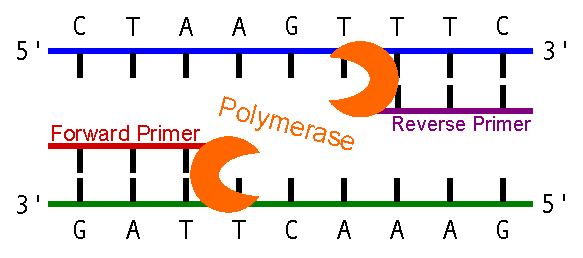
\includegraphics[width=\textwidth]{graphics/PCR.eps}
         \caption{A basic depiction of PCR, with polymerase in orange, forward
                  primer in red, and reverse primer in purple.}
         \label{fig:pcr}
      \end{figure}

      Polymerase chain reaction (PCR) is applied to the DNA being analyzed
      prior to pyrosequencing. PCR is a necessary first step
      for many types of DNA analysis and sequencing methods. Typically, PCR is
      used for DNA amplification, a process for making millions of copies of a
      target DNA region. This ensures that perturbations or reactions that are
      necessary for DNA analysis methods to work produce a large, observable
      signal or product. While the details of the PCR process are not necessary
      for understanding pyrosequencing, it is necessary to know that the PCR
      process requires two, typically short, nucleotide sequences known as
      \textit{primers}. Conceptually, a forward primer binds to the left of the
      target DNA region on the bottom strand (typically depicted from 3' end to
      5' end) and a reverse primer binds to the right of the target DNA region
      on the top strand. The two primers ensure that the polymerase enzyme is
      able to bind to, and copy, the desired region of DNA being analyzed. This
      can be seen in Figure \ref{fig:pcr}. The importance of the primers is
      described in Section \ref{sec:representation}. After PCR has been
      applied, the DNA being analyzed is ready for pyrosequencing.

      \begin{figure}[b]
         \centering
         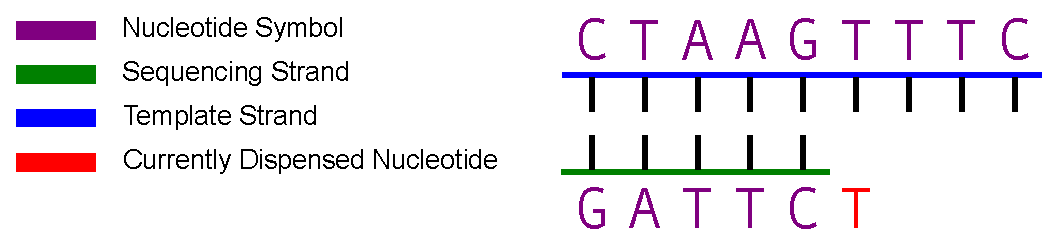
\includegraphics[width=\textwidth]{graphics/PyrosequencingComponents.eps}
         \caption{The parts of DNA during pyrosequencing.}
         \label{fig:pyrosequencing_legend}
      \end{figure}

      Pyrosequencing is a DNA sequencing process where a new strand of DNA,
      which we will refer to as the \textit{sequencing strand}, is built
      incrementally, complementary to the strand of DNA being sequenced, which
      we will call the \textit{template strand}. These components are
      highlighted in Figure \ref{fig:pyrosequencing_legend}. Ronaghi, et al.
      describe the pyrosequencing process in more
      detail~\cite{ronaghi:shedsLight}. This process takes place on a
      \textit{plate} containing many \textit{wells}--$24$ wells for the
      \textbf{PyroMark Q24}, a pyrosequencing machine manufactured by Qiagen
      pictured in Figure \ref{fig:pyromark} and currently in use by the Biology
      department at Cal Poly, San Luis Obispo. A pyrosequencing \textit{run}
      refers to the entirety of the pyrosequencing process for a single plate.
      While only one plate can be processed per run, each well on the plate
      contains a separate pyrosequencing reaction. For the PyroMark Q24, this
      means that a single run can pyrosequence 24 separate template strands.
      During a run, nucleotides--\textbf{A}denine, \textbf{T}hymine,
      \textbf{C}ytosine, or \textbf{G}uanine--are dispensed into each well of
      the plate.

      \begin{figure}[t]
         \centering
         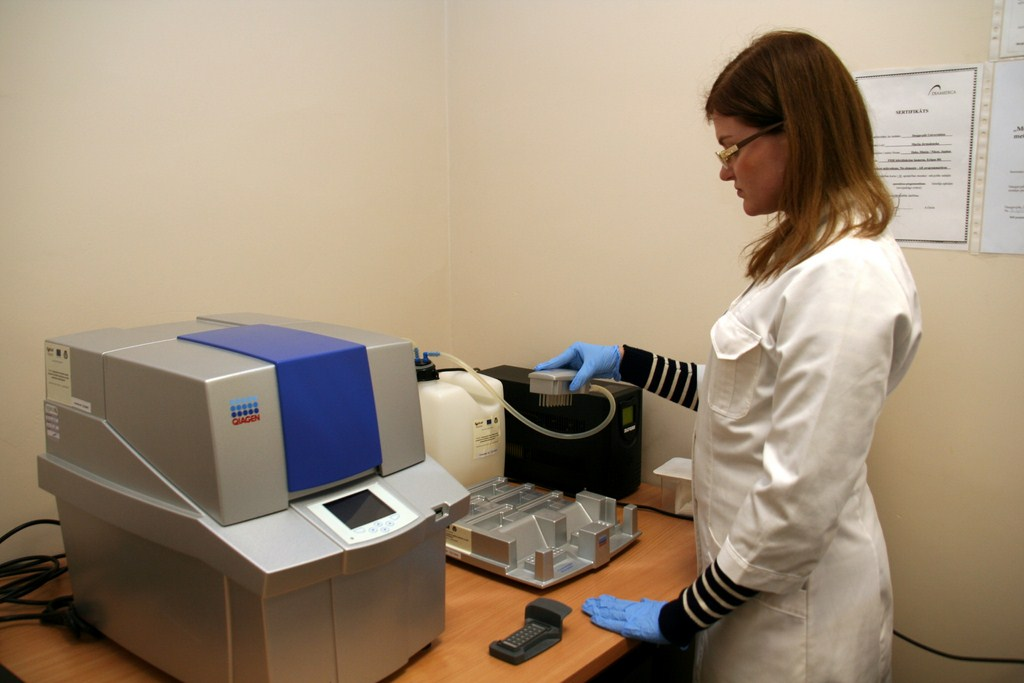
\includegraphics[width=0.4\columnwidth]{graphics/PyroMarkQ24.eps}
         \caption{[placeholder]The Qiagen PyroMark Q24 pyrosequencer.}
         \label{fig:pyromark}
      \end{figure}

      The order in which nucleotides are dispensed is determined by
      a parameter called the \textit{dispensation sequence}. Once a nucleotide is
      dispensed, it binds with the next available unbound nucleotide of the
      template strand if, and only if, they are complementary--\textbf{A} binds
      with \textbf{T} and \textbf{C} binds with \textbf{G}. If the dispensed
      nucleotide binds to the template strand, the sequencing strand is
      extended and light is emitted. Any remaining nucleotide not incorporated
      is enzymatically destroyed and the next nucleotide in the dispensation
      sequence is dispensed. When the dispensed nucleotide is incorporated into
      the sequencing strand, the observed light emittance is proportional to
      the amount of nucleotides incorporated into the sequencing strand, as
      seen in Figure \ref{fig:pyrosequencing}. For example, if \textbf{G} is
      incorporated into the sequencing strand and the light emittance is
      measured at 100 units and \textbf{T} is incorporated into the sequencing
      strand with light emittance 300 units, then the template strand has three
      times as many \textbf{T} nucleotides following a series of \textbf{G}
      nucleotides. When pyrosequencing, these proportions can be used to
      directly figure out the content of the template strand. However, as
      further described in Section \ref{sec:pyroprinting}, this is not true for
      pyroprinting.

      \begin{figure}[t]
         \centering
         \begin{subfigure}[t]{0.45\textwidth}
            \centering
            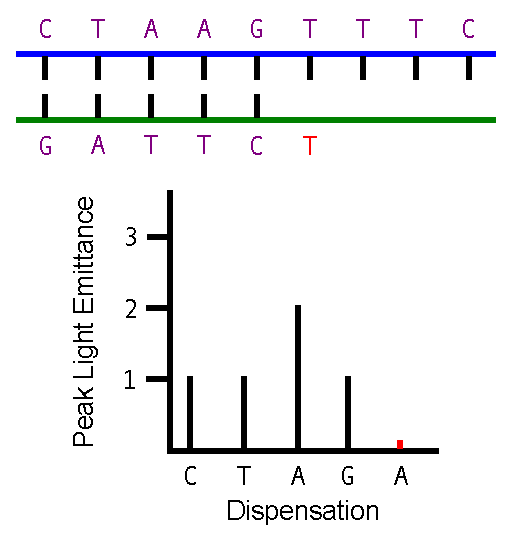
\includegraphics[width=\textwidth]{graphics/Pyrosequencing_NotIncorporated.eps}
            \caption{No light is emitted when the dispensed nucleotide is not
                     incorporated into the sequencing strand.}
            \label{fig:not_incorporated}
         \end{subfigure}
         \hfill
         \begin{subfigure}[t]{0.45\textwidth}
            \centering
            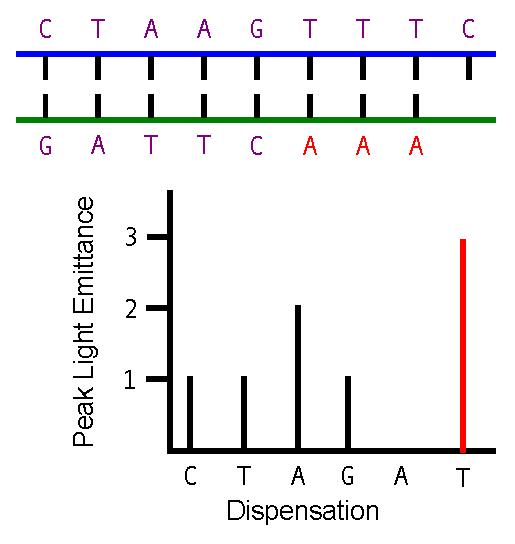
\includegraphics[width=\textwidth]{graphics/Pyrosequencing_Incorporated.eps}
            \caption{The light emitted when the dispensed nucleotide is
                     incorporated into the sequencing strand is proportional to
                     the amount of nucleotides incorporated.}
            \label{fig:incorporated}
         \end{subfigure}
         \caption{Depictions of pyrosequencing and the construction of a
                  pyrogram.}
         \label{fig:pyrosequencing}
      \end{figure}

      \begin{figure}[t]
         \centering
         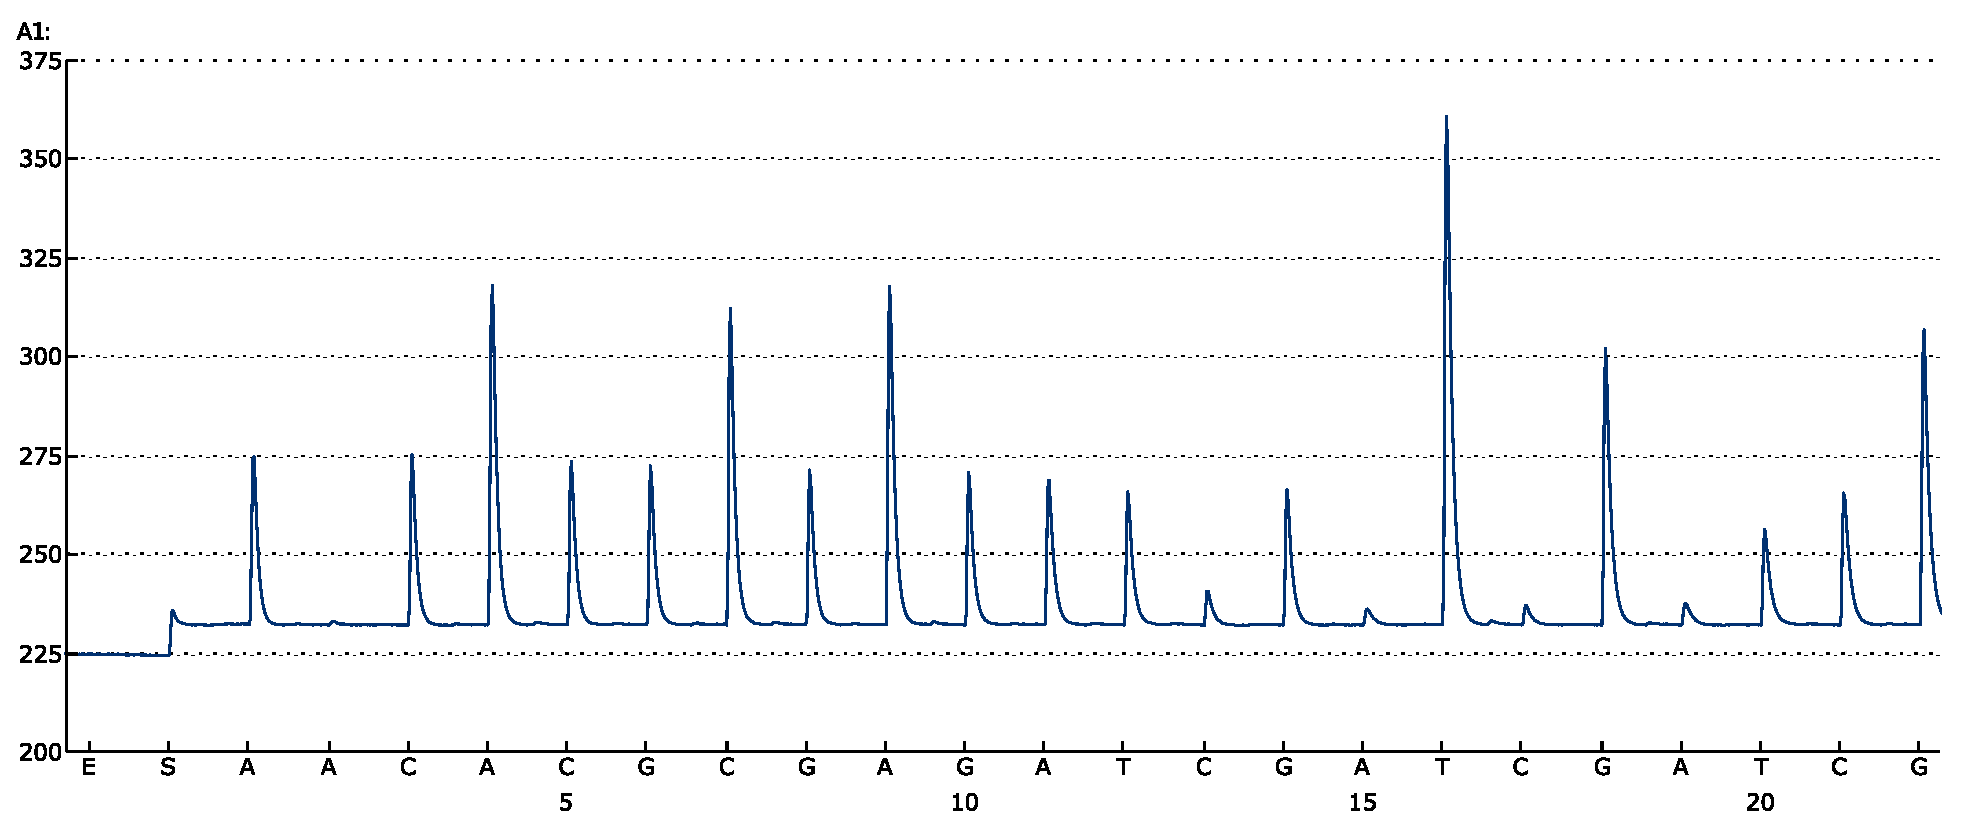
\includegraphics[width=\columnwidth]{graphics/pyrogram.eps}
         \caption{A pyrogram up to dispensation 22 (out of 104). The y-axis is
                  light emittance, the x-axis is dispensation over time.}
         \label{fig:pyrogram}
      \end{figure}

      \begin{figure}[t]
         \centering
         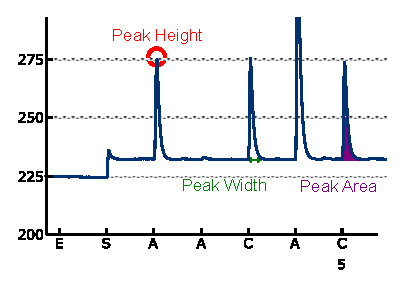
\includegraphics[width=0.65\columnwidth]{graphics/pyrogram_annotated.eps}
         \caption{A pyrogram annotated with peak height, peak width, and peak area.}
         \label{fig:annotated_pyrogram}
      \end{figure}

      The pyrosequencing machine measures the light emitted from the binding
      reaction of the dispensed nucleotide and the template DNA strand. The
      light emittance is then recorded as discrete values starting at the
      moment of dispensation. Light emittance is recorded until the moment when
      the chemical reaction between the dispensed nucleotide and the template
      strand completes. These light emittance values are used to construct a
      \textit{pyrogram}, a graph that plots light emittance of DNA synthesis
      against units of time and the dispensation sequence. In the pyrogram
      pictured in Figure \ref{fig:pyrogram}, light emittance (y-axis) is
      plotted against moments, which fall within a dispensation. When a
      nucleotide is dispensed, the light emitted increases rapidly in the
      initial moments, then subsides as the reaction completes.

      Each light emittance value recorded during the reaction corresponds to a
      \textit{moment}--a unit of time that is defined internally to either the
      pyrosequencer software or hardware. Each moment is associated with the
      dispensed nucleotide actively reacting in the well. For the purposes of
      analysis, three scalar light emittance values are associated with each
      dispensation, and so a pyrogram is abstractly similar to a histogram.
      Figure \ref{fig:annotated_pyrogram} show three distinct properties of the
      light emittance values recorded during each dispensation which are used
      to represent pyrosequencing results:
      \begin{itemize}
         \item Peak Height -- The maximum light emittance during a dispensation
         \item Peak Width -- The amount of time light was emitted during a
                             dispensation.
         \item Peak Area -- The total amount of light emitted during a
                            dispensation.
      \end{itemize}
      For the work in this thesis, peak height is used as the light emittance
      value for each dispensation. Based on brief studies, the biologists
      decided that peak height is the preferred light emittance value and so
      peak width and peak area, while maintained in the database, were not used
      for analysis.

      Modern pyrosequencing equipment allows for dispensation sequences of up
      to 200 nucleotides in length, however, the quality of the sequencing
      process deteriorates beyond 100--120 dispensations. The reasons for this
      deterioration include build up of enzymes and chemicals in the well,
      hardware error such as splashes, human error in plate preparation, and
      others. For longer DNA sequences, overlapping reads of 100--120
      nucleotides must be made and assembled together.

      Although there is sequencing technology cheaper and capable of longer DNA
      sequence reads, known as next-generation sequencing
      (NGS)~\cite{Mardis:NGS}, newer sequencing technology has a high initial
      cost and is generally less academically accessible. Compared to other
      sequencing technologies with cheaper initial cost, however,
      pyrosequencing is a very cheap and quick method. Even though relatively
      cheap, the characterization of the population of bacterial strains of a
      particular environment via many 100--200 DNA sequence reads becomes
      expensive very quickly. For this reason, the Biology department adapted
      pyrosequencing to be cheaper yet more effective for strain
      differentiation purposes. This is done by pyrosequencing multiple strands
      of DNA in parallel in a single well. This process, pyroprinting,
      leverages the fact that introduced nucleotides will bind with the first
      available nucleotide of the template strand by sequencing multiple
      template strands in the same reaction. This is clear in the case where
      the template strands are identical (DNA amplification), but the template
      strands used in pyroprinting are not necessarily identical.

   \section{Pyroprinting}\label{sec:pyroprinting}
      Pyroprinting is an MST technique that generates pyroprints (DNA
      fingerprints) through the use of pyrosequencing. Constructed pyroprints
      are output from the pyrosequencer as pyrograms of light emittance per
      nucleotide dispensation based on the DNA from highly variable regions of
      the microbial genome. These regions, called \textit{intergenic
      transcribed spacers} (ITS), are non-coding regions of the genome located
      between two highly conserved genes. There are two ITS regions, shown in
      Figure \ref{fig:its_regions}, used in the analysis of \textit{E. coli}
      isolates in this thesis: 16S--23S and 23S--5S.

      \begin{figure}[t]
         \centering
         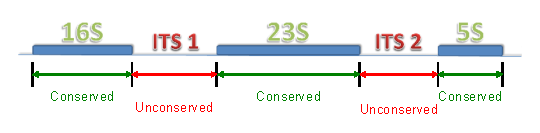
\includegraphics[width=\columnwidth]{graphics/ITS_regions.eps}
         \caption{A depiction of the 16S, 23S, 5S genes and their contained ITS
                  regions.}
         \label{fig:its_regions}
      \end{figure}

      For MST, the 16S--23S ITS region, located between the 16S and 23S genes,
      is a widely used ITS region for identifying bacterial
      strains~\cite{Boyer:ITS, Roth:Phylo, Tyler:Primers}. Although less
      commonly used, the 23S--5S ITS region is another well-known ITS region.
      These ITS regions are used in pyroprinting by the Cal Poly Biology
      department because both of these regions of DNA are non-coding.
      Non-coding regions of DNA accumulate more variability, or mutations, than
      regions of DNA that code for important proteins due to the lack of
      selective pressures.

      While a pyrogram is typically constructed to represent the pyrosequencing
      of a single template strand, a pyroprint is constructed to represent the
      pyrosequencing of several, possibly different, template strands. As
      pictured in Figure \ref{fig:genome}, the \textit{E. coli} genome has
      seven copies of both the 16S--23S and 23S--5S ITS regions, each with
      potentially different DNA sequences. Example DNA sequences for the
      16S--23S and 23S--5S ITS regions are pictured in Figure
      \ref{fig:sample_ITS}. The 16S--23S ITS template strands are colored
      green, whereas the 23S--5S ITS template strands are colored blue.
      Further, nucleotide positions that vary between template strands are
      colored purple to show that the variability between replicates of the
      16S--23S ITS region differ from the variability between replicates of the
      23S--5S ITS region.

      \begin{figure}[t]
         \centering
         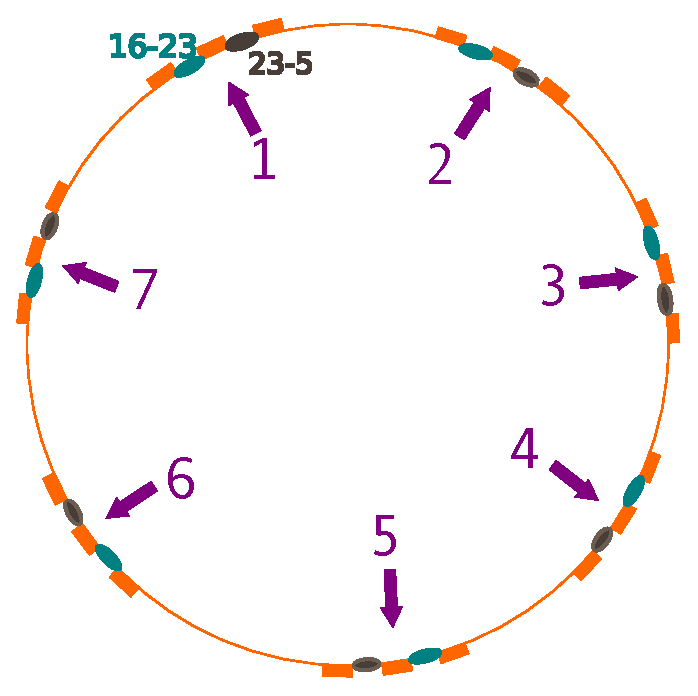
\includegraphics[width=0.45\columnwidth]{graphics/genome_with_highlighted_regions.eps}
         \caption{A depiction of a bacterial genome containing seven replicates
                  of the 16S--23S and 23S--5S ITS regions.}
         \label{fig:genome}
      \end{figure}

      \begin{figure}[t]
         \centering
         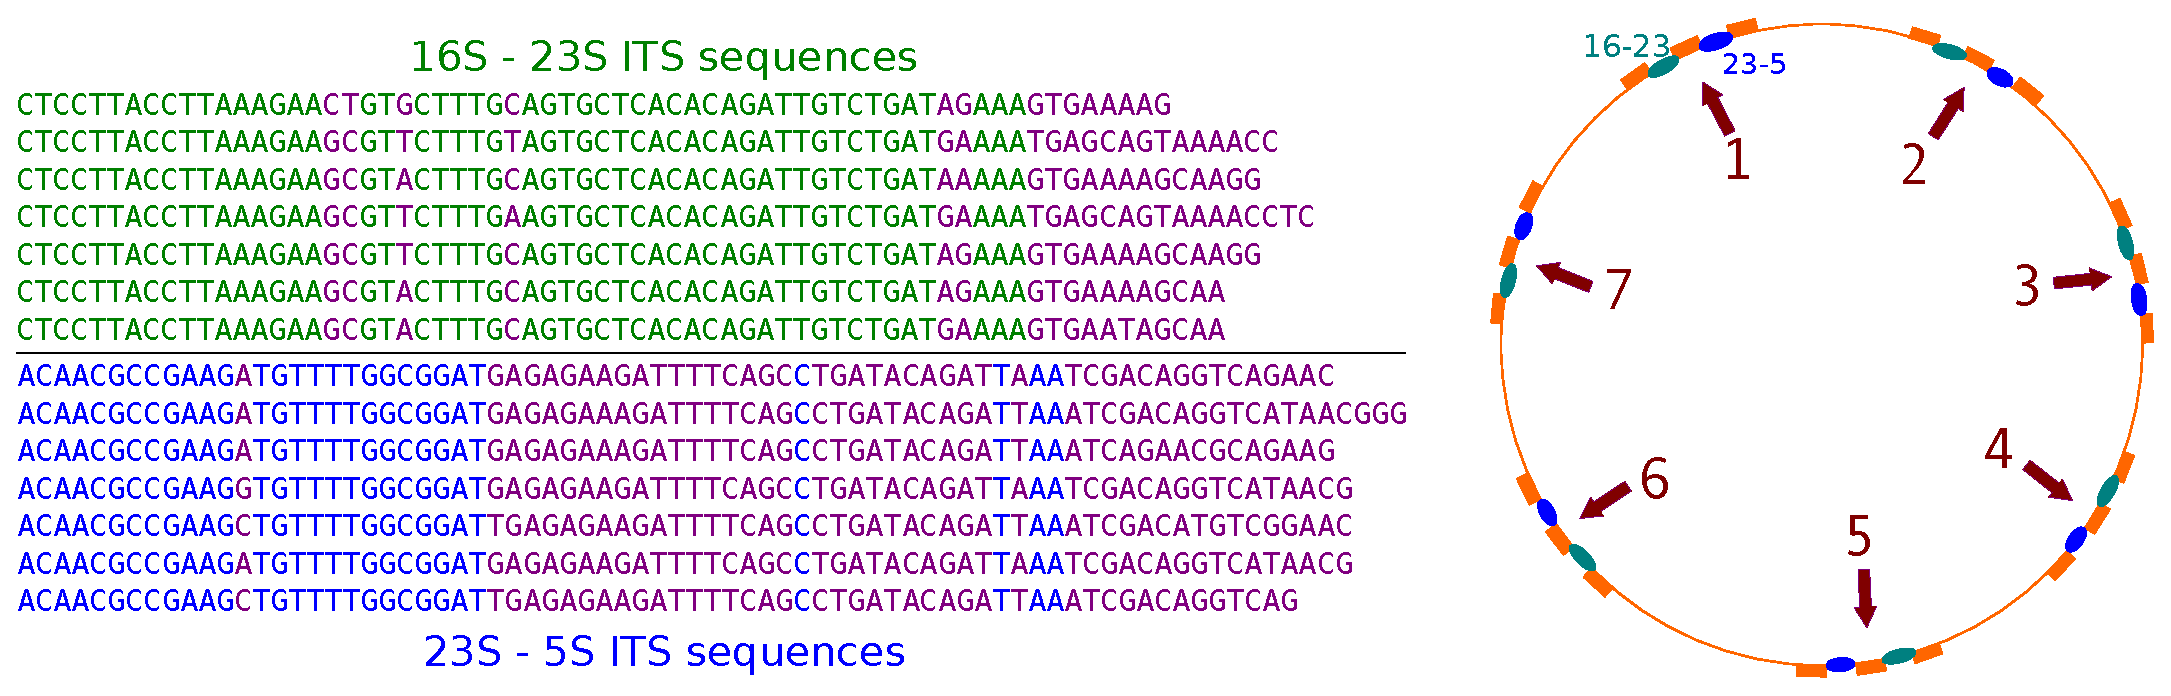
\includegraphics[width=\columnwidth]{graphics/sample_ITS_sequences.eps}
         \caption{Two sets of 7 DNA sequences that each come from a unique
                  replicate of the 16S--23S (green) and 23S--5S (blue) ITS
                  regions. Purple nucleotides symbolize nucleotides that vary
                  between replicates of an ITS region.}
         \label{fig:sample_ITS}
      \end{figure}

      The primary difference between pyroprinting and pyrosequencing is that
      pyrosequencing, using only one template strand, is used to determine the
      content of a DNA sequence. Pyroprinting, using multiple template
      strands, is unable to provide direct information regarding the content of
      DNA sequences. However, pyroprints represent an aggregate of several
      template strands, thus providing information about the variation between
      each template strand when compared to other pyroprints. The variation in
      the ITS regions can manifest between ITS regions of different bacterial
      isolates and also between ITS region replicates in the same genome. This
      variability can be observed as polymorphisms, or changes in a few or many
      nucleotides, in the DNA sequence. Each ITS region has varying degrees of
      variability depending on the choice of FIB. By pyrosequencing multiple
      template strands in a single well, pyroprinting effectively uses the
      several copies of each ITS region present in the microbial genome to
      create useful DNA fingerprints despite the length limitation of
      pyrosequencing reads. In other words, pyroprints are constructed such
      that each pyroprint is an aggregate of several, possibly different,
      template strands.

      The pyroprinting process and the use of several template strands is
      depicted in Figure \ref{fig:pyroprint_example}. Template sequences are
      pictured at the top of the figure, while the pyroprint is pictured at the
      bottom of the figure. Nucleotides in the template strand that are not
      fully sequenced by the example dispensation sequence are crossed out with
      a black line. The colored lines between nucleotides in the template
      sequences show what nucleotides in the template strand are bound to
      dispensed nucleotides as dispensations occur. The colored bars in the
      pyroprint at the bottom are to make it easy to relate the light emitted
      during a dispensation to the corresponding position in the template
      sequences.

      \begin{figure}[t]
         \centering
         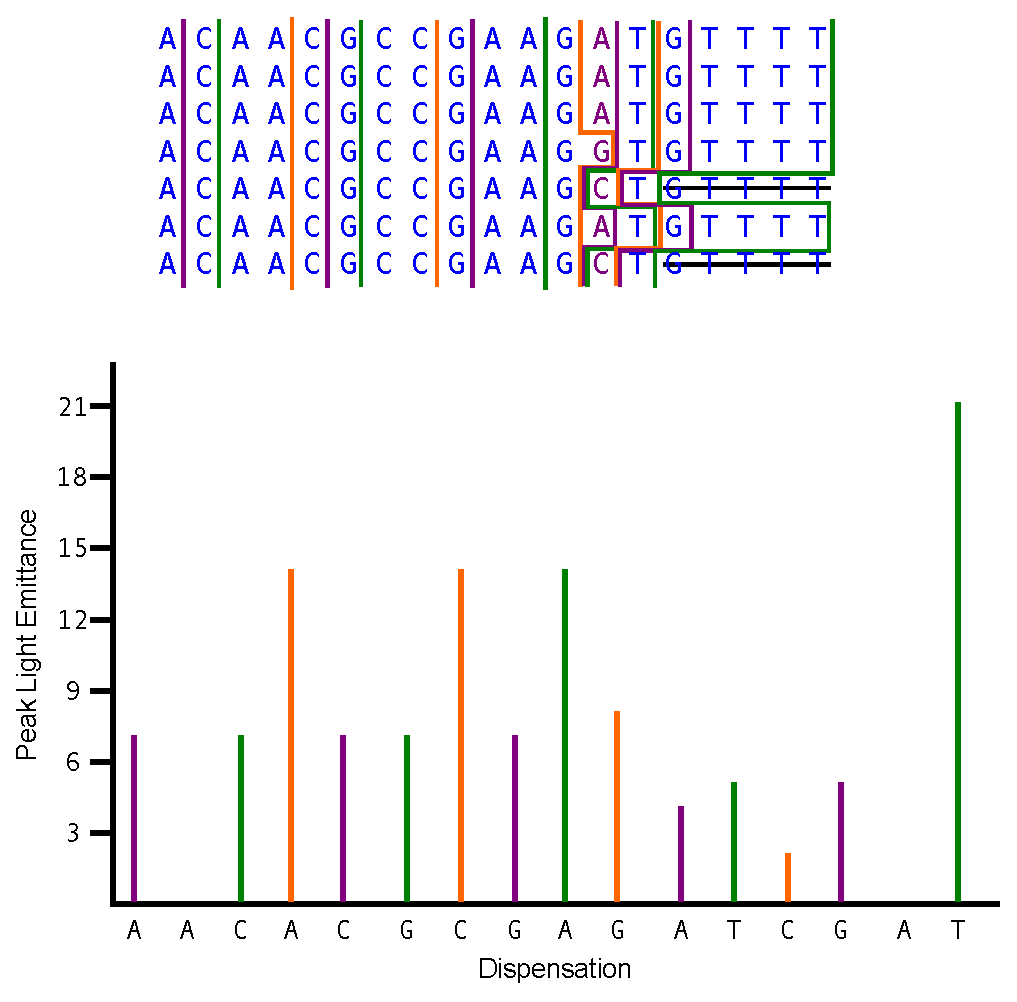
\includegraphics[width=0.70\columnwidth]{graphics/PyroprintExample.eps}
         \caption{An example pyroprint constructed from seven 23S--5S ITS
                  sequences.}
         \label{fig:pyroprint_example}
      \end{figure}

      \section{Data and Digital Representation}\label{sec:representation}
      In this thesis, the term \textbf{data point} is used to refer to a
      singular, usually complex, object. More generally, a data point is an
      individual record or object of data that can be compared and grouped with
      other individual records or objects of data. Prior to this section,
      bacterial isolates, pyroprints, ITS regions, light emittance, and various
      other forms of information relevant to MST and pyroprinting were
      introduced and described. Typically, only bacterial isolates and
      pyroprints are complex entities of interest which we consider data
      points. In this section, the digital representations of these biological
      entities are described and mathematically defined.

      There are three primary biological entities being analyzed--bacterial
      isolates, ITS regions, and pyroprints. Isolates have several ITS regions
      of interest present in the genome, each ITS region may be pyroprinted
      multiple times, and pyroprints consist of many light emittance values and
      a dispensation sequence. Computationally, bacterial isolates are
      represented as an object containing a set of ITS regions. An ITS region
      is a set containing pyroprints constructed from the ITS region. A
      pyroprint consists of a nucleotide sequence co-indexed with a vector of
      floating point values, representing light emittance values. While
      pyroprints serve as the basis on which bacterial isolate similarity is
      determined, the relationships between pyroprints and bacterial isolates
      is important for computing meaningful and appropriate similarities.

      When comparing biological entities, it is important that the comparison
      only be made in a biologically meaningful context. For example,
      \textit{E. coli} isolates should only be compared to other \textit{E.
      coli} isolates. Since bacterial isolates are individuals of a chosen FIB,
      it is only meaningful to compare bacterial isolates of the same FIB. For
      pyroprints, there is a quintuple (5-tuple) of parameters that should be
      identical for the comparison to be biologically meaningful. The 5-tuple
      of parameters is called a \textit{protocol} and represents the context in
      which pyroprints were constructed. Formally, a protocol is defined as
      follows:
      $$\mathcal{T} = \langle R, d, Pr_{f}, Pr_{r}, Pr_{s} \rangle$$
      The ITS region $R$ determines the actual DNA being targeted for the
      pyroprinting process. Ultimately the other four variables are determined
      so that PCR and pyrosequencing can be applied to the desired section of
      the ITS region. The dispensation sequence $d$ determines the order in
      which nucleotides are introduced in the pyrosequencing process. The
      significance of the dispensation sequence is detailed in Section
      \ref{sec:pyroprintdat}. The forward and reverse primers $Pr_{f}$ and
      $Pr_{r}$, respectively, are primers chosen for PCR prior to pyroprinting.
      The sequencing primer $Pr_{s}$, is a primer used for synthesis as part of
      the pyrosequencing process. Each parameter that is part of the protocol
      $\mathcal{T}$ is very important and affects the DNA content from which a
      pyroprint is constructed. If the protocols for pyroprints being compared
      differ from each other, then the comparison between the two pyroprints is
      completely meaningless.

      To capture the relationships and properly represent all three entities,
      we use the following mathematical notation:
      $$\mathcal{I} = \{I_1, \ldots, I_n\}$$
      $$\mathcal{R} = \{R_1, \ldots, R_k\}$$
      $$\mathcal{P} = \langle \mathcal{T}, \{\langle I_1, p_1 \rangle, \ldots,
                      \langle I_m, p_m \rangle \} \rangle,$$
      where $\mathcal{I}$ represents the set of all bacterial isolates in the
      input dataset and $\mathcal{R}$ represents the set of all ITS regions
      that can be found in the genome of the FIB being studied. While we
      represent ITS regions in such a way that it is possible to have any
      number $k$, the work in this thesis only considers $k=2$ ITS regions:
      $R_1 =$ ``$16-23$'' and $R_2 =$ ``$23-5$''. The set of all pyroprints,
      $\mathcal{P}$, is represented as a triple consisting of:
      \begin{itemize}
         \item The dispensation sequence used for pyrosequencing ($d$)
         \item An ITS region of origin ($R$)
         \item A set of all bacterial isolate-pyroprint pairs ($\{\langle I_m,
               p_m\rangle\}$) such that $I_m$ is the bacterial isolate of
               origin from which pyroprint $p_m$ was constructed.
      \end{itemize}
      The pyroprint $p_m$ is then represented as a tuple of the form:
      $$p = \langle d, \bar{p}\rangle$$
      where $d$ and $\bar{p}$ are both represented as vectors:
      $$d = (d_1, \ldots, d_n) \qquad d_i \in \{A, T, C, G\}$$
      $$\bar{p} = (p_1, \ldots, p_n) \qquad p_i \in \mathds{R}_0^+$$
      Such that $d$ is a dispensation sequence. Each light emittance value
      $p_i$ of a pyroprint $\bar{p}$ may be any positive real number or $0$.
      The work in this thesis only explores the use of peak light emittance
      values for each dispensation and does not consider peak width or peak
      area. For brevity, pyroprint light emittance vectors are referred to as
      pyroprint vectors.

   \section{Similarity Metric}\label{sec:sim_metric}
      For the comparison of pyroprints, assuming the protocols for each are
      identical, Pearson's correlation is the similarity metric of choice. If
      the protocol for each pyroprint differs, a default similarity of $-2$ is
      produced. This ensures that bacterial isolates with different protocols
      cannot possibly be grouped together, and the result, since it is outside
      the possible range of Pearson's correlation, also signifies that the
      comparison was not computed. Pearson's correlation is a similarity
      metric formulated in the following way for two pyroprints $\bar{p}$ and
      $\bar{q}$:
      $$
         sim(\bar{p},\bar{q}) =
         \frac{
            \sum_{i=1}^{n}{(p_i - E(\bar{p})) \: (q_i - E(\bar{q}))}
         }
         {
            \sqrt{\sum_{i=1}^{n}(p_i-E(\bar{p}))} \:
            \sqrt{\sum_{i=1}^{n}(q_i-E(\bar{q}))}
         }
      $$
      For this formulation, $E(p)$ is the expected value, or mean, of the
      pyroprint vector $p$ such that:
      $$E(\bar{p}) = \frac{\sum_{i=1}^{n}{p_i}}{n}$$
      While this is the standard formulation of Pearson's correlation, it
      requires two passes over the pyroprint vector and is computationally
      expensive. Fortunately, there is an alternative formulation used in this
      thesis that can be computed in a single pass over the pyroprint vector:
      $$
         sim(\bar{p},\bar{q}) =
         \frac{
            (N\sum_{i=1}^{n}{p_i \, q_i}) -
            (\sum_{i=1}^{n}{p_i} \, \sum_{i=1}^{n}{q_i})
         }
         {
            \sqrt{N \sum_{i=1}^{n}{p_i^2} - (\sum_{i=1}^{n}{p_i})^2}
            \:
            \sqrt{N \sum_{i=1}^{n}{q_i^2} - (\sum_{i=1}^{n}{q_i})^2}
         }
      $$
      Pearson's correlation is the preferred similarity metric because
      pyrosequencing machines observe fluctuations in the amplitude of light
      emitted during binding reactions in the sequencing process. The reasons
      for these fluctuations can be contributed to hardware issues or
      inconsistencies in the PCR process of DNA amplification. These
      fluctuations are accommodated by comparing the variance between the two
      pyroprint vectors instead of a series of direct comparison between
      components of each pyroprint vector.

      The similarity between the same ITS region, $R_i$, of two bacterial
      isolates, $I_j, I_k$, is then computed as an aggregation of all pairwise
      Pearson's correlations computed between pyroprints in both ITS regions.
      The results shown in Chapter \ref{chap:evaluation} are computed using an
      average aggregation of pairwise Pearson's correlations as formulated
      here:
      $$
         R_{i}^{a} = \{p_{1}^{a}, \ldots, p_{s_{j}}^{a}\}^{\rightarrow I_{a}}
      $$
      $$
         R_{i}^{b} = \{p_{1}^{b}, \ldots, p_{s_{k}}^{b}\}^{\rightarrow I_{b}}
      $$
      $$
         sim(R_{i}^{a}, R_{i}^{b}) =
         \operatorname*{average}_{\substack{x \in [1,s_{j}]\\y \in [1, s_{k}]}}
                 (sim(p_{x}^{a}, p_{y}^{b}))
      $$
      The similarity between two bacterial isolates, $I_{\alpha}, I_{\beta}$,
      is then computed as the average of the similarities computed between each
      ITS region pair or $0$ if the similarity between any ITS region pair is
      too low:
      %$$
      %   sim(I_{a}, I_{b}) =
      %   \begin{dcases}
      %      0 & when\; sim(R_{16-23}^{a}, R_{16-23}^{b}) < \beta\\
      %      0 & when\; sim(R_{23-5}^{a}, R_{23-5}^{b}) < \beta\\
      %      \operatorname*{average}_{\substack{i \in \{16-23, 23-5\}}}
      %      (sim(R_{i}^{a}, R_{i}^{b})) & otherwise
      %   \end{dcases}
      %$$
      $$
         sim(I_{a}, I_{b}) = \operatorname*{average}_{
                                 \substack{i \in \{16-23, 23-5\}}
                             } (sim(R_{i}^{a}, R_{i}^{b}))
      $$
      The comparison of bacterial isolates is shown in (comparison figure to
      come).
      %TODO Figure \ref{fig:comparison}.


   \section{Bacterial Strains and Clusters}\label{sec:strains}
      Bacterial strains are a biological concept that describes a group of
      biologically related bacterial isolates. Informally, bacterial strains
      are groups of bacterial isolates that have very similar genotypes.
      Clusters are a computational concept that describes a group of highly
      related, or similar, entities. While bacterial strains have a specific
      biological context, clusters are very abstract and applicable to many
      different data. In this section, the connection between bacterial strains
      and clusters is explained so that the work described in this paper is
      clearly understood.

      Formally, a bacterial strain is a set of bacterial isolates, where the
      genotypes of each bacterial isolate has a high level of similarity to the
      genotype of each other bacterial isolate in the set. Pyroprints function
      as DNA fingerprints, representing each replicate of an ITS region. This
      makes pyroprints the perfect vehicle for determining the similarity of
      genotypes for a pair of bacterial isolates. The definition of a
      bacterial strain is given by the following notation:
      $$\mathcal{S} = \{S_1, \ldots, S_m\}$$
      $$S = \{I_1, \ldots, I_n\}$$
      Here, $\mathcal{S}$ represents the set of all determined strains $S_1$ to
      $S_m$. Using the similarity function $sim(I_{a}, I_{b})$ described in Section
      \ref{sec:sim_metric}, determining which bacterial isolates, $\{I_1,
      \ldots, I_n\}$, belong to each strain, $\{S_1, \ldots, S_m\}$, is done by
      incorporating bacterial isolates with a high similarity into the same
      strain $S_i$. It is from this definition that the problem of identifying
      bacterial strains can be clearly seen as a clustering problem. A direct
      parallel can be made between the biological concept of bacterial strains
      and the computational concept of clusters. In this way, the
      interpretation of constructed clusters is straightforward--each cluster
      corresponds to a \textit{potential} bacterial strain. Although the
      concept of a bacterial strain is directly represented by clusters, since
      there is no guarantee that a cluster represents a real bacterial strain,
      it can only be inferred that an observed cluster \textit{may} represent a
      bacterial strain, or at least closely resemble one. Described further in
      Chapter \ref{chap:algorithm}, bacterial isolates are grouped into
      clusters using either \textsf{agglomerative hierarchical clustering} or
      \textsf{OHClust!}

      When grouping bacterial isolates into bacterial strains, it is difficult
      to determine when two bacterial isolates are considered the same or
      ``similar enough.'' However, by definition, a bacterial strain must
      consist of bacterial isolates that are highly similar. And, equivalently,
      a cluster must contain data points that are highly similar. Therefore, it
      is necessary to formally define what ``highly similar'' means. ``Highly
      similar'' is typically defined by a threshold which is determined based
      on statistical or empirical properties of the data. Intuitively, we use
      thresholds to qualify whether the similarity between two data points is
      high enough to warrant grouping them together, or low enough to guarantee
      that they should not be grouped together. Nearly all clustering methods
      apply thresholds to similarity functions to ensure that only data points
      that are above, or meet, the threshold are clustered together. In this
      way, bacterial isolates will be associated with a bacterial strain if,
      and only if, they have genotypes at least as similar as an established
      threshold.

      \begin{figure}[t]
         \centering
         \begin{subfigure}[t]{0.45\textwidth}
            \centering
            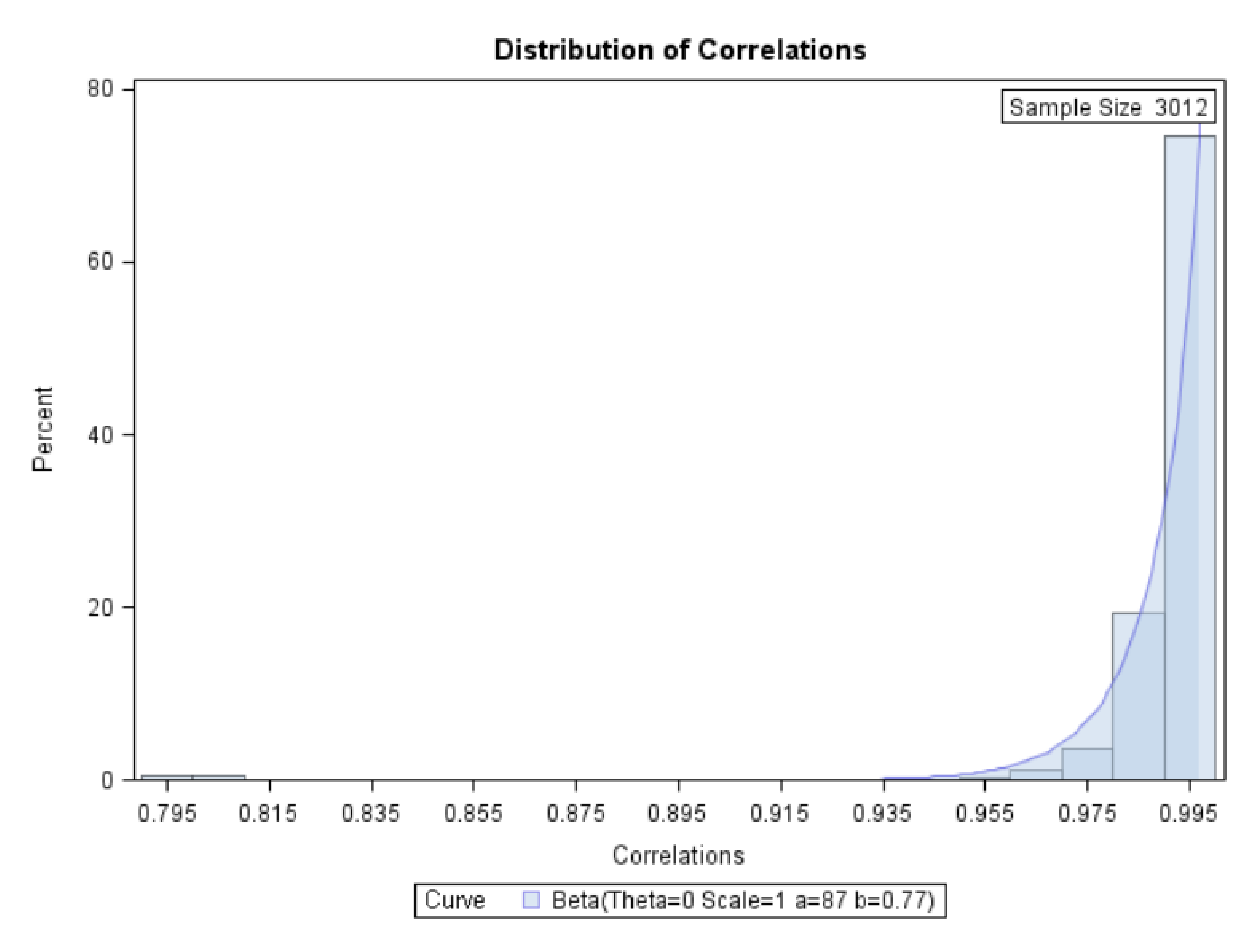
\includegraphics[width=\textwidth]{graphics/BetaDist_Match.eps}
            \caption{A beta distribution fit over comparisons between bacterial
                     isolates that would be considered definitely similar.}
            \label{fig:beta_match}
         \end{subfigure}
         \hfill
         \begin{subfigure}[t]{0.45\textwidth}
            \centering
            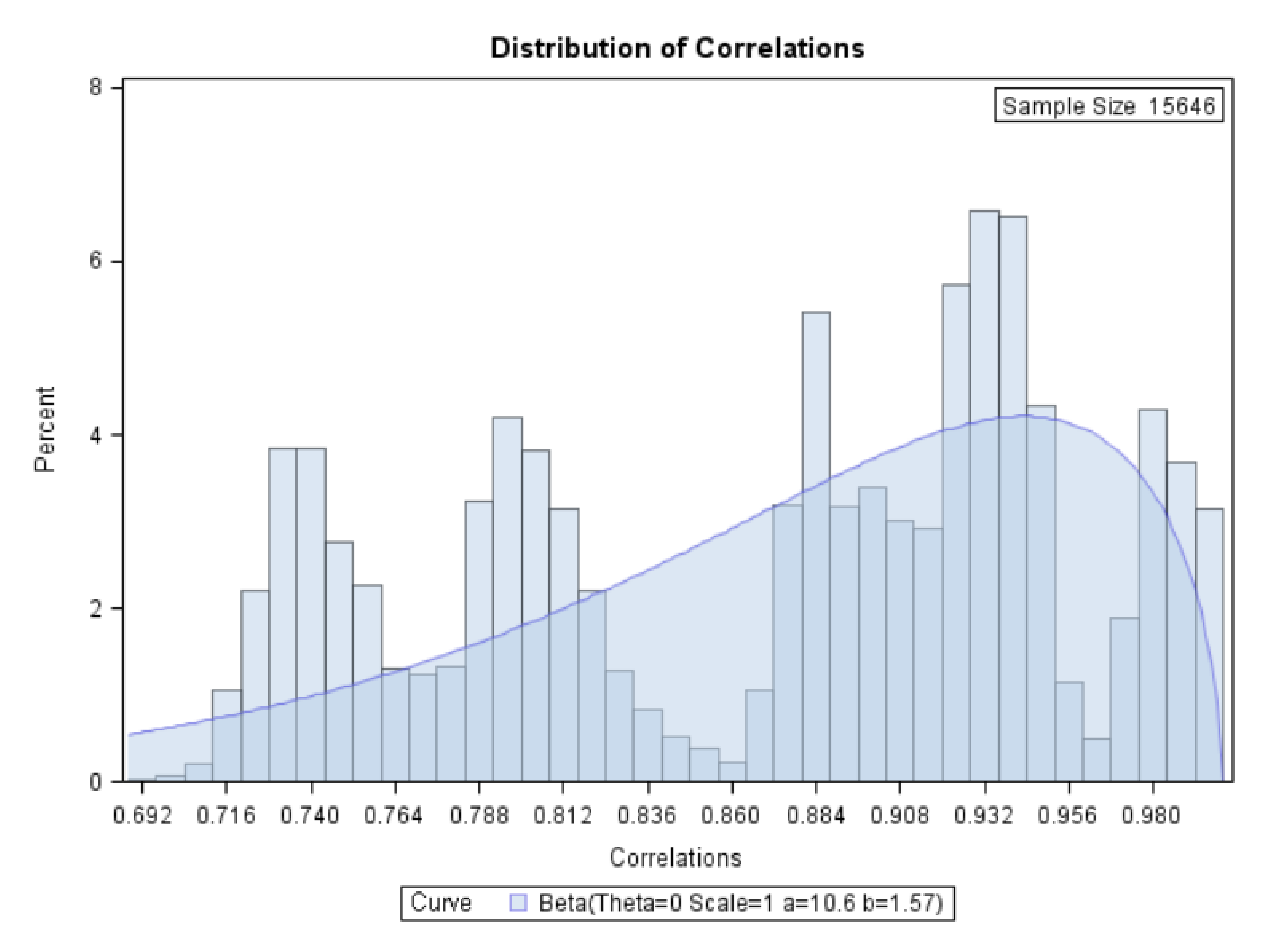
\includegraphics[width=\textwidth]{graphics/BetaDist_Mismatch.eps}
            \caption{A beta distribution fit over comparisons between bacterial
                     isolates that would be considered definitely dissimilar.}
            \label{fig:beta_mismatch}
         \end{subfigure}
         \caption{Beta distributions fit over comparisons between bacterial
                  isolates that are either definitely similar or definitely
                  dissimilar.}
         \label{fig:match_mismatch}
      \end{figure}

      \begin{figure}[t]
         \centering
         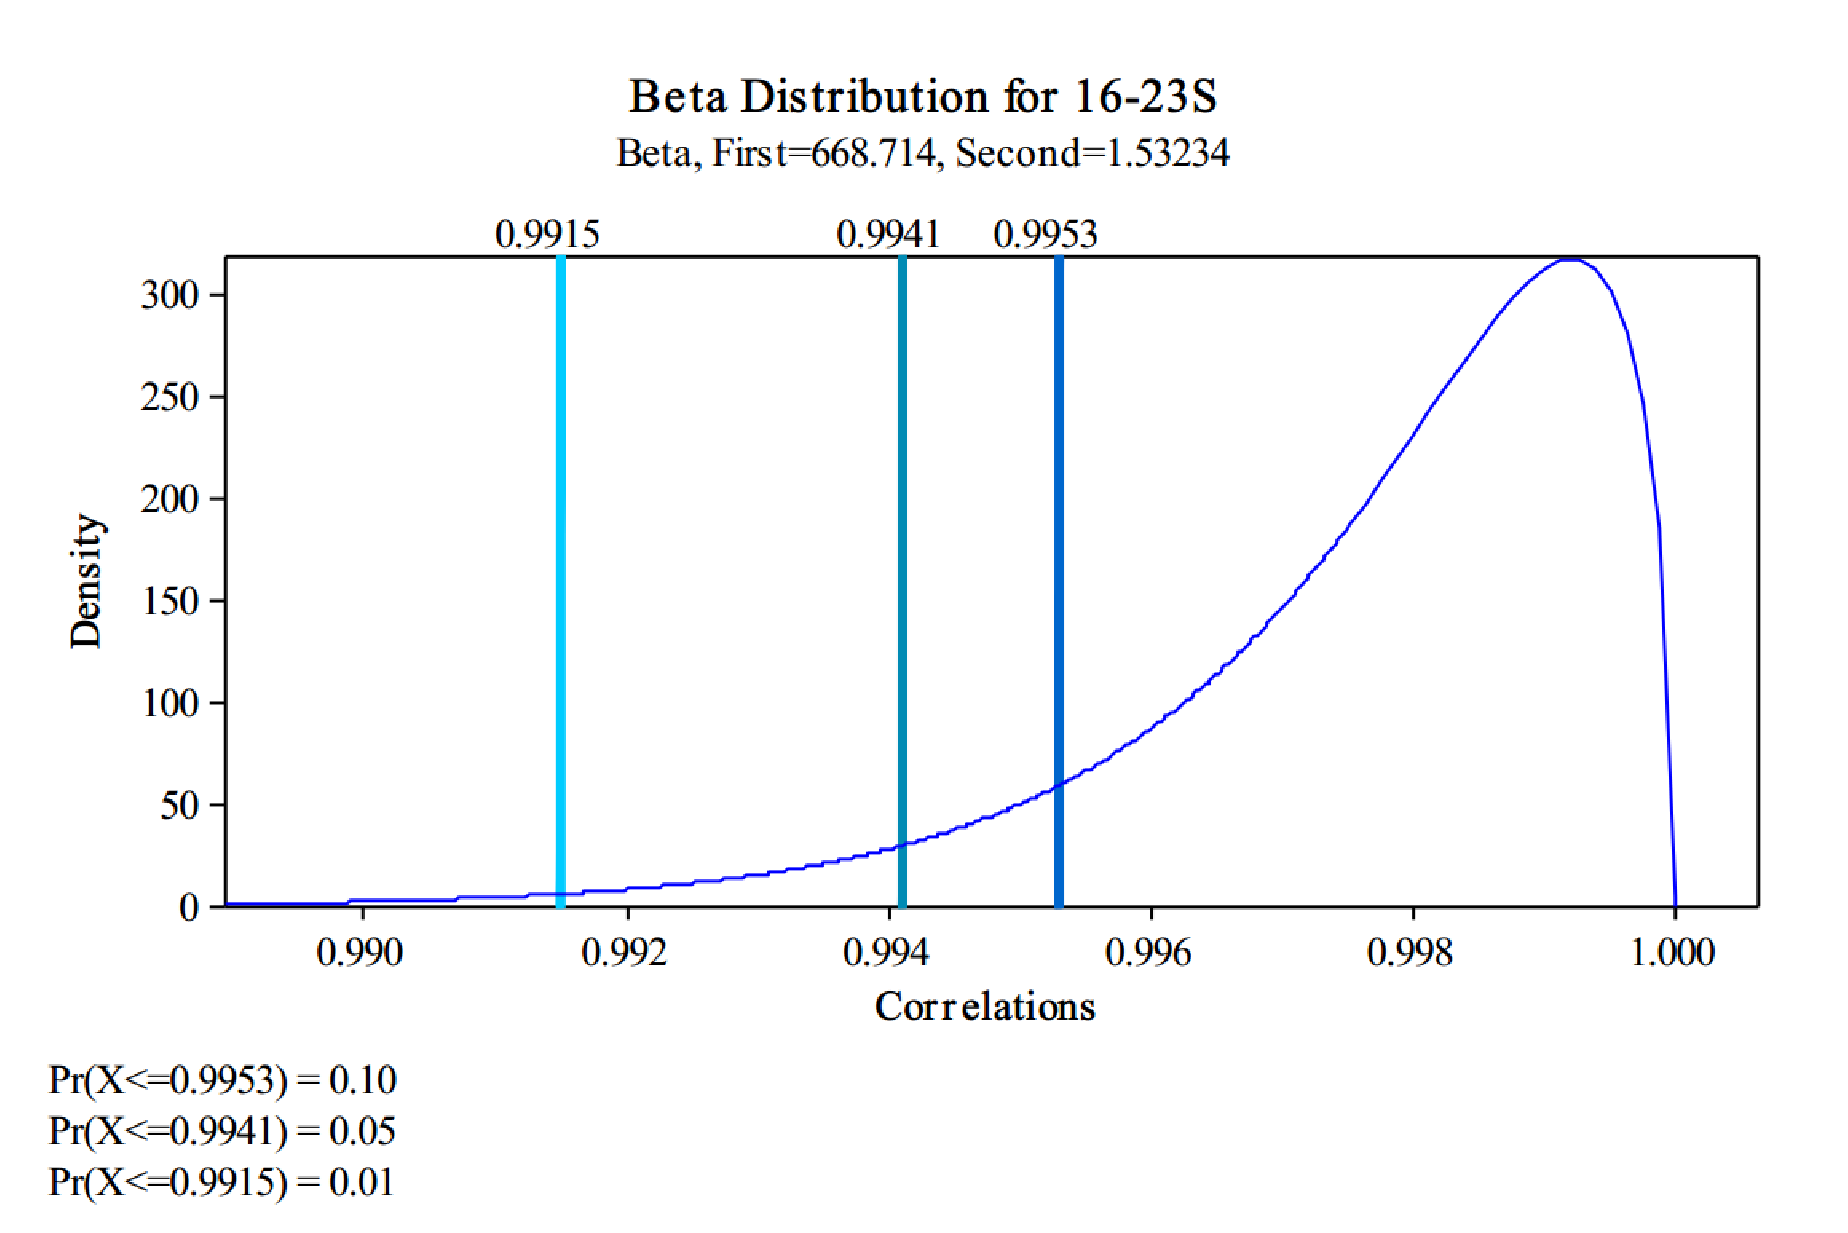
\includegraphics[width=0.70\columnwidth]{graphics/BetaDist16-23.eps}
         \caption{A beta distribution fitted onto comparisons between
                  pyroprints constructed from the 16S--23S ITS regions of
                  bacterial isolates from pidgeons for a statistical
                  experiment.}
         \label{fig:beta_16}
      \end{figure}

      \begin{figure}[t]
         \centering
         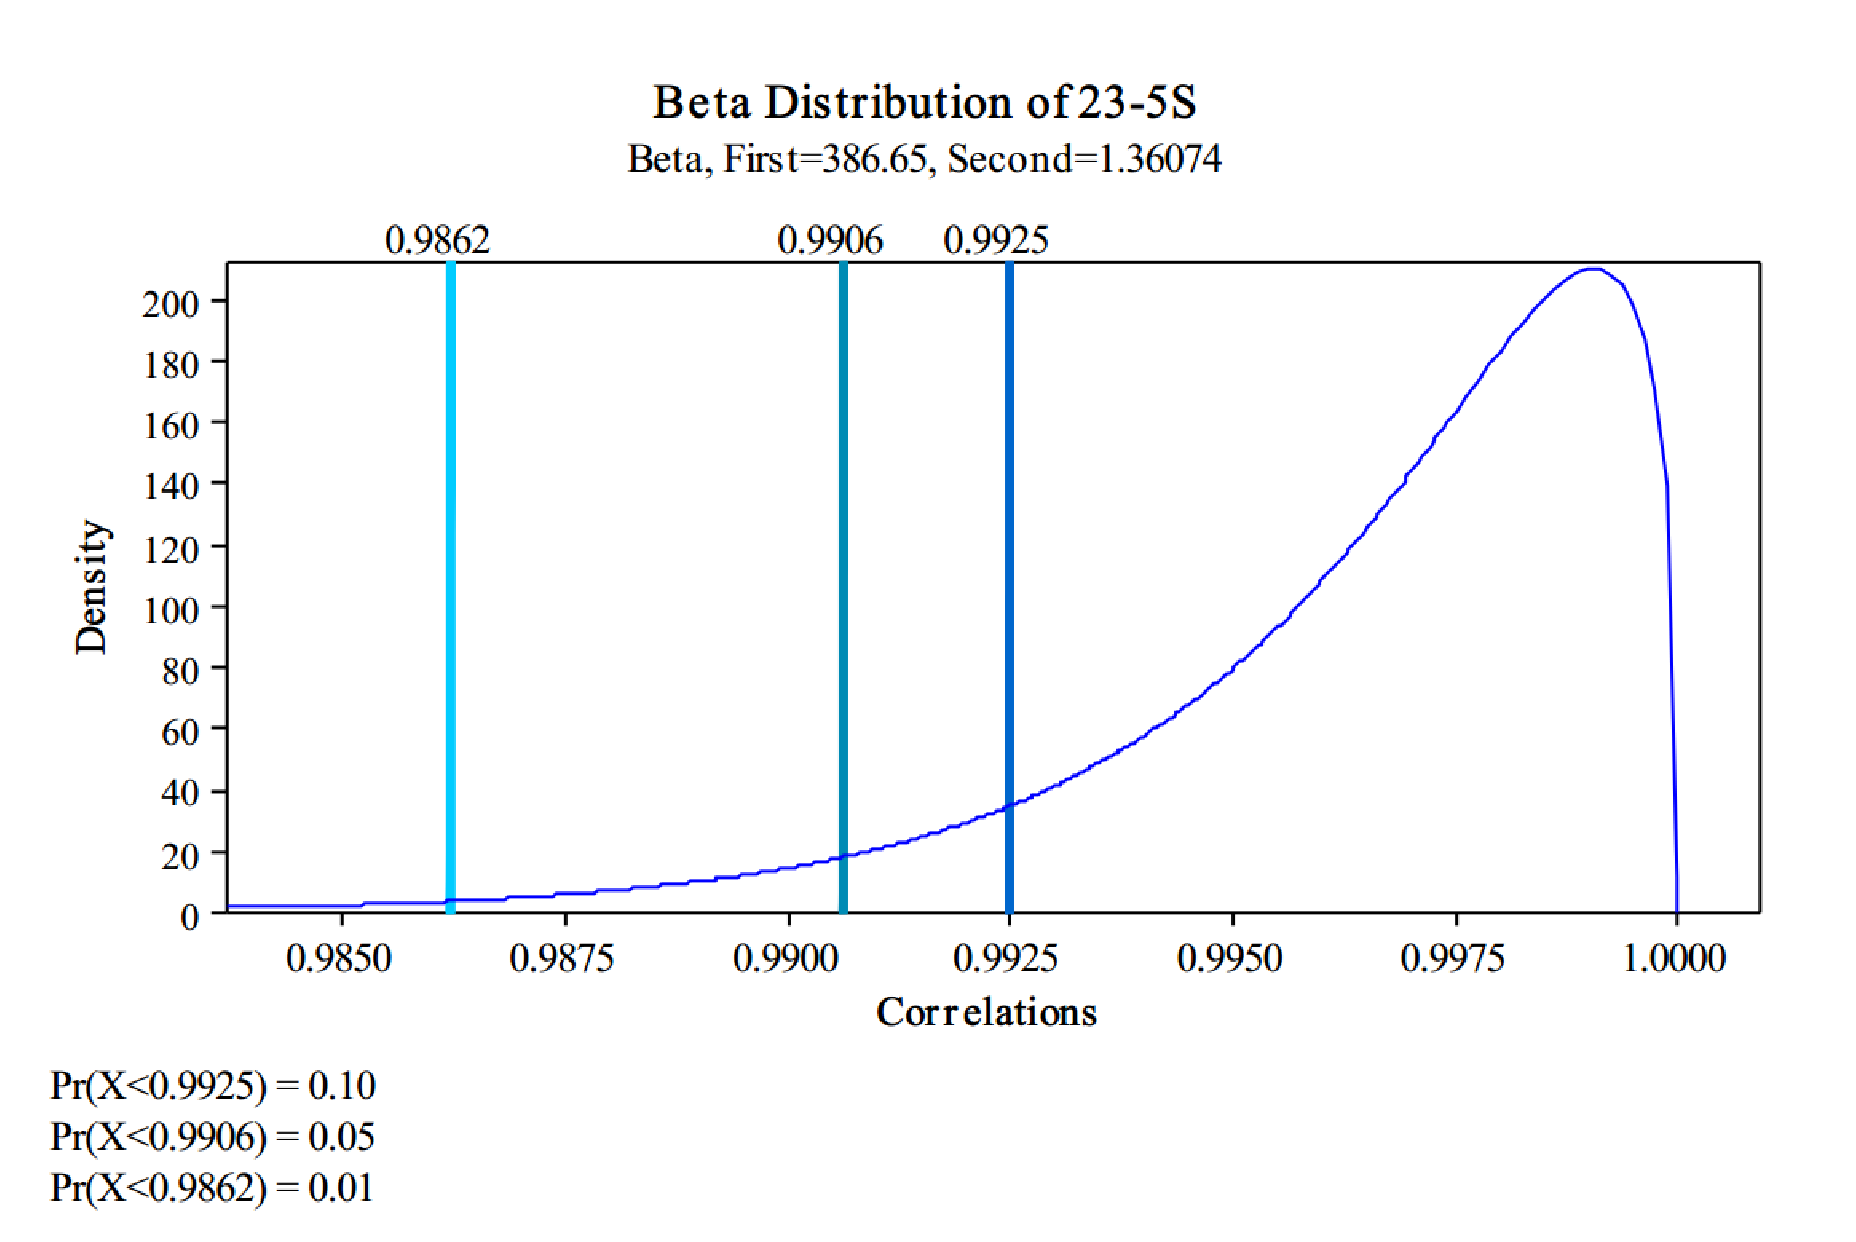
\includegraphics[width=0.70\columnwidth]{graphics/BetaDist23-5.eps}
         \caption{A beta distribution fitted onto comparisons between
                  pyroprints constructed from the 23S--5S ITS regions of
                  bacterial isolates from pidgeons for a statistical
                  experiment.}
         \label{fig:beta_23}
      \end{figure}

      A statistics student, Diana Shealy, has conducted a statistical
      study~\cite{Shealy:SeniorProject} using a dataset of bacterial isolates
      that were pyroprinted multiple times in multiple ITS regions. The
      study was conducted to investigate appropriate threshold values for
      interpreting pyroprint similarities as one of three categories:
      \begin{itemize}
         \item Definitely similar
         \item Definitely dissimilar
         \item Reasonably similar but possibly a false-positive or
               false-negative. Colloquially referred to as ``squishy.''
      \end{itemize}
      To categorize pyroprint comparisons as one of these three categories, two
      thresholds were established during Diana's statistical study. The upper
      threshold $\alpha$ defines a minimum similarity for pyroprints to be
      considered definitely similar. Alternately, the lower threshold $\beta$
      defines a maximum similarity for pyroprints to be considered definitely
      dissimilar. Between these two thresholds, pyroprint similarity seems to
      suggest similarity between their associated bacterial isolates, but
      increases the likelihood of false positives and false negatives.

      For the statistical study, a likelihood ratio approach was initially
      taken. For this approach, pyroprint similarities that were considered
      definitely similar or definitely dissimilar were separated into two
      groups. For each group, pictured in Figure \ref{fig:match_mismatch}, a
      beta distribution was fit to the data. Unfortunately, it was determined
      that the distribution of dissimilar pyroprint similarities is not
      constant for all combinations of different samples, while the
      distribution of similar pyroprint similarities is. This lead to Diana
      having to take an approach other than likelihood ratio.

      The alternate approach to determining threshold values for pyroprint
      similarity was to find a beta distribution that closely fit the
      distribution depicted in Figure \ref{fig:beta_match}. Interestingly,
      pyroprints that were constructed from the same bacterial isolate and that
      fit the same distribution, seemed to fit the same distribution as
      pyroprints constructed from a different bacterial isolate that correlated
      with other pyroprints from that bacterial isolate. That is, for a given
      bacterial isolate, pyroprints that correlated with each other fit the
      same distribution as pyroprints for a different bacterial isolate.
      Leveraging this information, Diana then determined Pearson's correlation
      values that resembled common rejection regions. The common rejection
      regions, shown in Figure \ref{fig:beta_16} for the 16S--23S ITS region
      and Figure \ref{fig:beta_23} for the 23S--5S ITS region, represent
      regions where the amount of false negatives are $1$\%, $5$\%, and $10$\%.
      For this analysis, a false negative refers to two bacterial isolates that
      are from the same bacterial strain but are associated with different
      bacterial strains. With consideration of the results of the statistical
      study for both the 16S--23S and 23S--5S ITS regions, the biologists have
      currently decided to use two threshold values, $\alpha = 0.995$ and
      $\beta = 0.99$. For the 16S--23S ITS region, this means having a $10$\%
      false negative rate. For the 23S--5S ITS region, this means having an
      even higher false negative rate. However, the statistical study
      fit beta distributions to distributions of pyroprint similarities for a
      single ITS region. By using both the 16S--23S and 23S--5S ITS regions
      together for determining similarity, the false negative and false
      positive rate is ideally significantly lower. Unfortunately, there has
      not been enough time or man-power to investigate the actual false
      negative and false positive rates when considering both ITS regions in
      conjunction.

      Although only two threshold values are used in this thesis, $\alpha =
      0.995$ and $\beta = 0.99$, it is important to note that thresholds will
      vary depending on ITS region and the FIB being studied. Following the
      aforementioned statistical study, it was decided that for research
      conducted so far with \textit{E. coli}, it is acceptable to use the same
      $\alpha$ and $\beta$ thresholds for both 16S--23S and 23S--5S ITS
      regions. However, thresholds are handled in a generic way and so the work
      described in this thesis is not restricted to using these threshold
      values.

   \section{Clustering}\label{sec:clustering}
      There are many datasets where relationships may exist that are not easily
      observable to the human eye. The analysis of data based on similarity
      functions determined by various relationships is known as cluster
      analysis, clustering, or unsupervised
      learning~\cite{Jain:DataClustering}. Phrased another way, clustering is
      the organization of a collection of patterns, or data points, based on
      similarity. The groups or partitions that are formed during clustering
      are referred to as \textit{clusters}. Clustering is used for the analysis
      of many different types of data and although it can be done many ways,
      there are two primary families of clustering algorithms--hierarchical and
      partitional.

      Partitional clustering algorithms iteratively assign and re-assign data
      points to cluster centroids or seeds. A cluster centroid is a single data
      point selected to represent the ``center'' of a cluster. Centroids are
      initially selected from random or maximally distant data points. Then, on
      each iteration of the algorithm, data points are assigned to the closest
      centroid. At the end of each iteration, the data point that is closest to
      the center of the cluster becomes the cluster centroid. The method used
      to assign data points to cluster centroids during each iteration
      differentiates many partitional algorithms. \textsf{K-means clustering}
      approaches this by assigning data points to the cluster of the closest
      centroid on each iteration. For \textsf{k-means clustering}, clusters are
      mutually exclusive and when a data point is assigned to a cluster, it is
      removed from its previous cluster. Generally, due to the use of
      centroids, partitional clustering algorithms are most effective when
      there is a general idea of how many partitions exist in the input
      dataset. For the required analysis of pyroprinting, for which there is no
      clear idea of how many partitions exist, partitional clustering
      algorithms are not very useful, and therefore not explored further,
      except in Chapter \ref{chap:related}~\cite{Jain:DataClustering}.

      Hierarchical clustering algorithms take an approach that considers every
      data point a cluster and approaches data analysis in a pairwise manner.
      Iteratively, pairs of clusters that are maximally similar are grouped,
      or, alternatively, clusters that are maximally dissimilar are separated.
      Unlike partitional clustering algorithms, hierarchical clustering
      algorithms do not re-assign data points to different clusters on later
      iterations. Since hierarchical clustering does not use centroids when
      clustering, the order of clustering is deterministic for a fixed
      dataset.

      \begin{figure}[t]
         \centering
         
\includegraphics[width=0.7\columnwidth]{graphics/DendogramExample.eps}
         \caption{A dendogram representing clusters for a dataset of seven data
                  points. Numbers correspond to most similar data points.}
         \label{fig:dendogram_example}
      \end{figure}

      Clustering decisions made by hierarchical clustering, which clusters
      should be joined to form a new cluster, are maintained in a binary tree
      called a \textit{dendogram}. A dendogram represents clusters as internal
      nodes, or connections, and represents data points as the bottom-most
      points of the tree. An example of a dendogram is shown in Figure
      \ref{fig:dendogram_example}. The numbers on the left mark a point in the
      dendogram when two data points or clusters join to form a new cluster.
      Each colored part of the dendogram corresponds to a colored data point
      pictured at the bottom. Data points are clustered together from highest
      similarity (corresponding to the node marked $1$) to lowest similarity
      (corresponding to the node marked $6$). Once the dendogram is constructed
      and the entire dataset forms a single cluster, desirable clusters can be
      determined by making a ``cut'' in the dendogram. A cut is depicted in
      Figure \ref{fig:dendogram_example_with_cut} between the fourth and fifth
      clusters. A cut represents a point at which similarities between data
      points or clusters must be above (below as pictured in the Figure) in
      order to be considered an acceptable cluster. Similarities that are below
      the similarity marked by the cut are ignored and data points or clusters
      are not joined. The example shown in Figure
      \ref{fig:dendogram_example_with_cut} shows three clusters were formed:
      \begin{itemize}
         \item the cluster formed with the fourth highest similarity
         \item the cluster formed with the third highest similarity
         \item the data point that has the least similarity to the other
               clusters.
      \end{itemize}
      Since hierarchical clustering algorithms do not require any knowledge of
      how many partitions may exist in the dataset, this is the type of
      clustering algorithm further explored for analysis of
      pyroprints~\cite{Jain:DataClustering}.

      \begin{figure}[t]
         \centering
         
\includegraphics[width=0.7\columnwidth]{graphics/DendogramExample_WithCut.eps}
         \caption{A dendogram with a cut made above the fourth highest
                  similarity, forming three separate clusters.}
         \label{fig:dendogram_example_with_cut}
      \end{figure}

      \subsection{Agglomerative Hierarchical Clustering}\label{sec:agglomerative}
         \textsf{Agglomerative hierarchical clustering}, or
         \textsf{agglomerative clustering} for short, is the standard
         bottom-up hierarchical clustering approach. \textsf{Agglomerative
         clustering} initially considers each data point as a cluster and joins
         the pair of clusters with the maximal similarity on every iteration.
         This is known as a bottom-up approach because the dendogram for the
         input dataset is built from the leaves--each data point--to the
         root--all data points clustered together. There are two primary
         components of \textsf{agglomerative clustering}: the similarity
         metrics used between data points and clusters, and the threshold for
         cutting the dendogram.

         \begin{figure}[t]
            \centering
            
\includegraphics[width=0.7\columnwidth]{graphics/ClusterMetrics.eps}
            \caption{A diagram of three cluster similarity functions.}
            \label{fig:cluster_metrics}
         \end{figure}

         The two primary similarity functions that must be computed during
         \textsf{agglomerative clustering} are: similarity between data points,
         and similarity between clusters. The similarity function between data
         points is determined independent of the clustering algorithm and is
         based on the data being analyzed. In contrast, similarity functions
         between clusters are chosen based on the relationships in the data
         that are being studied. While there are several cluster similarity
         functions that can be used, there are three cluster similarity
         functions, pictured in Figure \ref{fig:cluster_metrics}, that are
         typically used:
         \begin{itemize}
            \item Single-Link
            \item Complete-Link
            \item Average-Link
         \end{itemize}

         Each of the three listed cluster similarity functions yield clusters
         with very different properties. The single-link function computes
         similarity between clusters based on the similarity between the two
         closest points between the clusters. This function is preferable when
         data points have high similarity in a particular direction instead of
         equally high similarity in multiple directions. This can be seen in
         Figure \ref{fig:single_average_link} where the same dataset is shown
         to use single-link cluster similarity in Figure
         \ref{fig:good_single_link} and average-link in Figure
         \ref{fig:bad_single_link}. The average-link function computes
         similarity based on the average of each pairwise distance between each
         data point in the clusters being compared. This is easily shown in
         Figure \ref{fig:cluster_metrics} where there similarities between the
         outlying cluster and the middle cluster are used to calculate the
         average similarity between the two clusters. Referring back to Figure
         \ref{fig:good_single_link}, if the data points at the bottom of the
         black cluster were closer to the top data points in the greenish
         cluster, then single-link cluster similarity would be a bad choice
         because the whole dataset would form a single cluster. In such a case,
         average-link would be much better in order to observe a more wholistic
         relationship between clusters. In contrast to the single-link
         similarity function, the complete-link similarity function computes
         the similarity between two clusters based on the two data points that
         are most dissimilar, or least similar. This cluster similarity
         function is best used for datasets where very closely related clusters
         are desired. Understandably, complete-link is the most conservative
         cluster similarity function of the three mentioned functions. It is
         important to remember that ``good'' clusters are defined based on the
         dataset and the relationships being studied.

         \begin{figure}[t]
            \centering
            \begin{subfigure}[t]{0.45\textwidth}
               \centering
               
\includegraphics[width=\textwidth]{graphics/good_single_link.eps}
               \caption{An example of data that is better to use single-link
                        cluster similarity with.}
               \label{fig:good_single_link}
            \end{subfigure}
            \hfill
            \begin{subfigure}[t]{0.45\textwidth}
               \centering
               
\includegraphics[width=\textwidth]{graphics/bad_single_link.eps}
               \caption{An example of data that is better to use average-link
                        cluster similarity with.}
               \label{fig:bad_single_link}
            \end{subfigure}
            \caption{Possible clusterings using single-link or average-link
                     cluster similarity.}
            \label{fig:single_average_link}
         \end{figure}

         Once clustering is complete and a dendogram is constructed, the
         resulting set of clusters must still be determined. The dendogram is
         constructed only to provide an analysis of the relationships between
         the data points in the input dataset. Since the root of the dendogram
         always represents all data points of the dataset as a single cluster,
         there is a ``cut'' that must be made in the dendogram that determines
         at what point joining clusters is no longer meaningful. This point is
         called a threshold--a value, or level, that a similarity must exceed.
         Intuitively, the threshold can be described as the point at which two
         clusters are believed to contain highly related, or even identical,
         data points. This will have different interpretations depending on the
         data being analyzed and the objective of the analysis being carried
         out, and so is determined based on the input dataset. The dendogram
         cut is made across edges between internal nodes and child nodes.
         Dendogram nodes above the cut are ignored, and dendogram nodes
         directly below the cut are considered the final set of clusters. In
         this way it is plain that nodes lower in the dendogram have higher
         similarity between sub-clusters than nodes higher in the dendogram.

\chapter{Tools for Pyroprint Analysis}\label{chap:other_contributions}
   As part of the contributions of this thesis, there are two tools that
   address specific aspects of pyroprint analysis:
   \begin{itemize}
      \item A tool for analyzing the pyroprinting process \textit{in-silico},
            specifically for determining a preferred dispensation sequence.
      \item An interim tool used to analyze pyroprints prior to the creation of
            CPLOP~\cite{Jan:Thesis}, specifically to apply
            \textsf{agglomerative clustering} and a preliminary implementation
            of OHClust!.
   \end{itemize}
   The first tool, Pyroprint Dispensation Analysis Tool
   (\textit{PyroprintDAT}), provides analysis to assist in the selection of a
   dispensation sequence for pyroprinting. Unlike the typical pyrosequencing
   process, the use of several template strands for pyroprinting makes the
   choice of dispensation sequence important. The second tool is a tool for
   analyzing isolates and pyroprints given a similarity matrix of Pearson's
   correlations.

   \section{PyroprintDAT}\label{sec:pyroprintdat}
      PyroprintDAT provides biologists with the ability to pyroprint known DNA
      sequences \textit{in-silico} using a set of input dispensation sequences.
      It specifically addresses the goal of determining a ``best'', or most
      preferred, dispensation sequence for pyroprinting a population of bacterial
      isolates. Determining a best dispensation sequence for pyroprinting would be
      difficult and expensive if done \textit{in-vivo} or \textit{in-vitro}. By
      using PyroprintDAT for \textit{in-silico} analysis, the best dispensation
      sequence can be determined naively.

      Consider that pyroprinting is a technique for creating DNA fingerprints.
      Informally, the best kind of fingerprint is one that is most likely to
      differentiate between different individuals or identify correct bacterial
      strains. In consideration of this, a best dispensation sequence for
      pyroprinting can be informally understood as a dispensation sequence that
      makes pyroprints of bacterial isolates from different bacterial strains
      very different from each other. Since pyroprinting can yield different
      pyroprints based on the dispensation sequence used, it is desirable to
      determine the dispensation sequence that produces distinct pyroprints for
      bacterial isolates from different bacterial strains.

      \begin{figure}[t]
         \centering
         \begin{subfigure}[t]{0.45\textwidth}
            \centering
            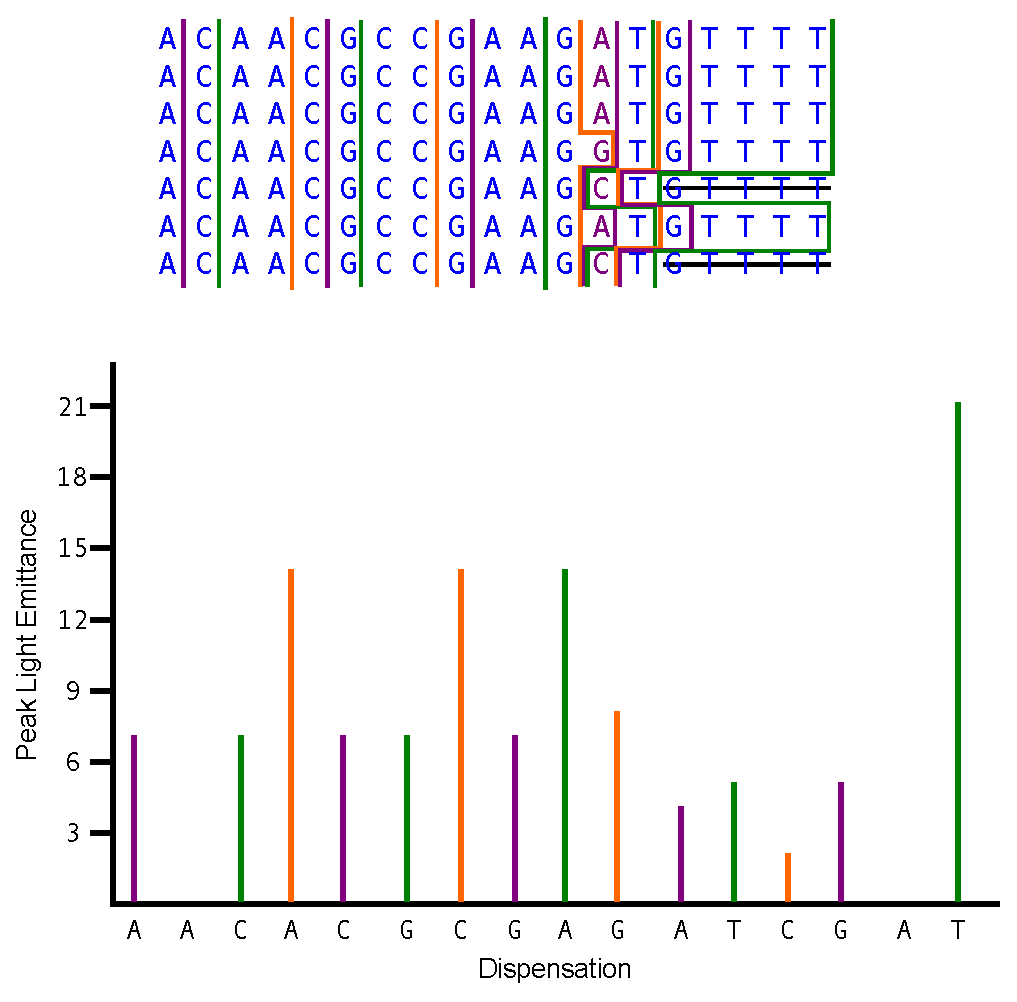
\includegraphics[width=\textwidth]{graphics/PyroprintExample.eps}
            \caption{A pyroprint with dispensation sequence AACACGCGAGATCGAT.}
            \label{fig:dispensation_example1}
         \end{subfigure}
         \hfill
         \begin{subfigure}[t]{0.45\textwidth}
            \centering
            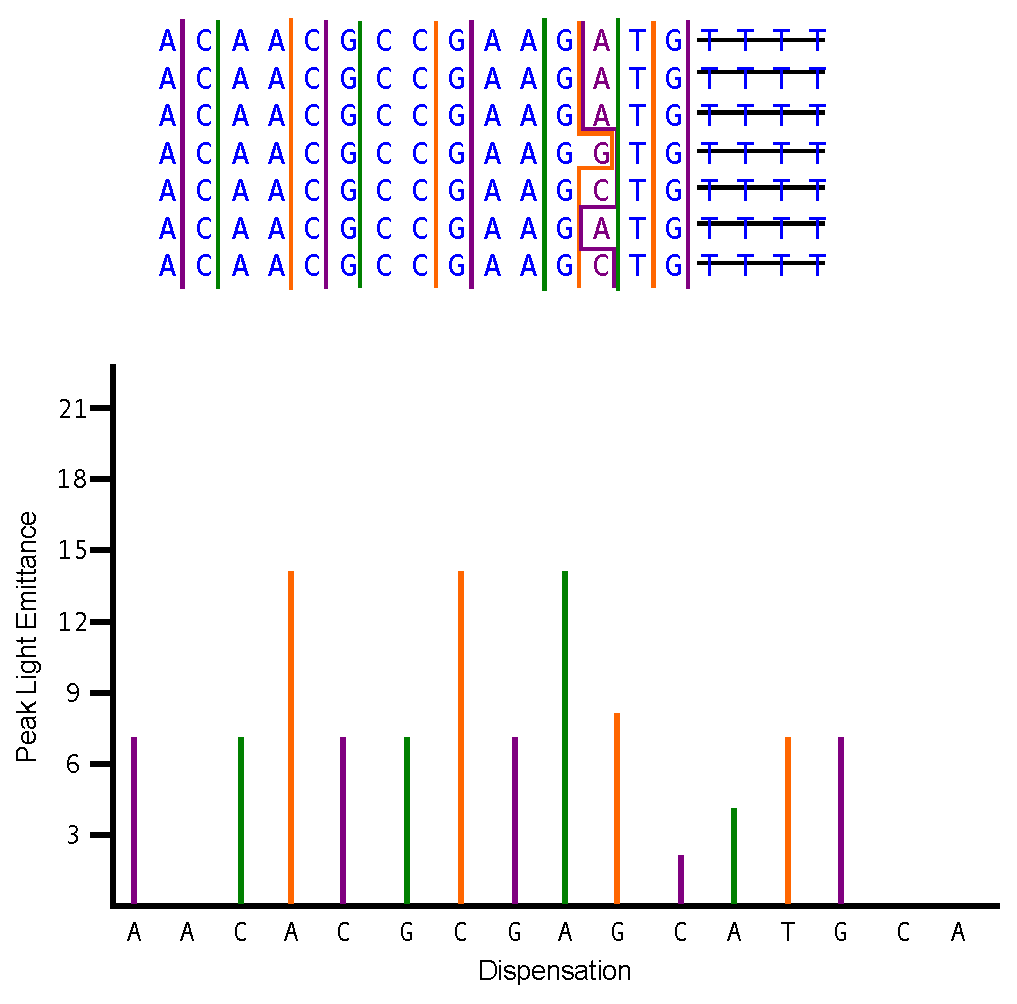
\includegraphics[width=\textwidth]{graphics/PyroprintExample2.eps}
            \caption{An alternate pyroprint with dispensation sequence
                     AACACGCGAGCATGCA.}
            \label{fig:dispensation_example2}
         \end{subfigure}
         \caption{Pyroprints using different dispensation sequences for the same
                  set of template strands.}
         \label{fig:dispensation_examples}
      \end{figure}

      Figure \ref{fig:dispensation_examples} shows two pyroprints produced by
      different dispensation sequences given the same set of template strands.
      Looking at the twelfth nucleotide in both figures
      \ref{fig:dispensation_example1} and \ref{fig:dispensation_example2}, it
      is clear that the pyroprinting process \textit{consumes} the template
      strands differently for the two dispensation sequences
      \textnormal{AACACGCGAGATCGAT} and \textnormal{AACACGCGAGCATGCA}. In order
      to best understand dispensation sequence analysis, it is important to
      have a clear understanding of how variable regions affect the
      pyroprinting process.

      \begin{figure}[t]
         \centering
         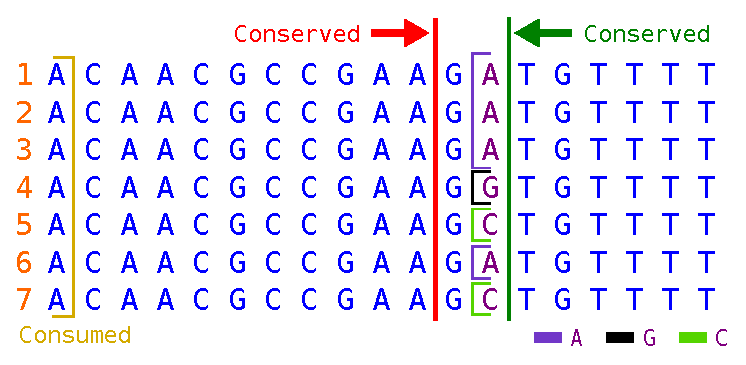
\includegraphics[width=0.7\columnwidth]{graphics/TemplateStrandAdvancement.eps}
         \caption{Annotated set of seven template strands. The red and green
                  lines mark the end and beginning of conserved regions,
                  respectively. Colored brackets mark corresponding nucleotides
                  in the variable region.}
         \label{fig:annotated_templates}
      \end{figure}

      Using Figure \ref{fig:annotated_templates} as a reference, consider each
      template strand independently. During the pyroprinting process, dispensed
      nucleotides react and bind with the next available nucleotide in a
      template strand. For multiple, independent template strands, this means
      that ``progress'' along each template strand will be consistent in
      conserved regions, but vary in unconserved regions. Biologically,
      progress is represented by the sequencing strand. As the sequencing
      strand incorporates more nucleotides, there are fewer available unbound
      nucleotides in the template strand. Computationally, progress can be
      conceptualized as a pointer advancing along a string. As a template
      strand is sequenced, a pointer advances.

      For example, a dispensation sequence that starts with \textbf{A}, will
      dispense a nucleotide that consumes the first nucleotide in template
      strands $1$ to $7$, shown as a gold bracket in Figure
      \ref{fig:annotated_templates}. For this example, the sequencing strand
      for each template strand has incorporated a single \textbf{T} nucleotide,
      and the pointer on each template strand is advanced one character.

      Until each sequencing strand reaches the end of the conserved region,
      marked by a vertical red line, each template strand is
      guaranteed to be consumed at the same rate. This means that for any
      dispensation sequence, the pyroprints for the first 11 nucleotides of
      the template strands will always be the same. Variations in pyroprints
      due to dispensation sequence begin to manifest to the right of the first
      conserved region. Between the two conserved regions, marked by red and
      vertical lines, there are two scenarios that can be considered.

      In one scenario, each template strand is consumed equally up to the green
      line, then each template strand is again consumed at the same rate in the
      conserved region. This scenario occurs if each \textbf{G}, \textbf{A},
      and \textbf{C} is consumed before the next nucleotide is dispensed to
      consume a \textbf{T}. This scenario is shown in Figure
      \ref{fig:dispensation_example2}.

      \begin{figure}[!t]
         \centering
         \fbox{\begin{minipage}{\textwidth}
            \begin{algorithmic}
               \Function{CompareSequences}{$D$, $F$}
                  \Comment{D: disp seqs, F: DNA in FASTA}

                  \State $BestDisp \gets null$
                  \Comment{value of best dispensation sequence}

                  \State declare $M[\;][\;][\;]$
                  \Comment{three dimensional array}

                  \For {$d_n \in D$}
                  \Comment {For each disp seq being considered}
                     \State $P \gets [\;]$

                     \For {$f_m \in FastaFiles$}
                        \Comment {For each FASTA DNA seq}
                        \State $P[m] \gets$ \textsf{CreatePyroprint}($f_m$)
                     \EndFor

                     \For {$i \in P[\;]$}
                     \Comment{$M$ gets similarity matrix for $d_n$}
                        \For {$j \in P[\;]$}
                           \State $M[n][i][j] \gets$ \textsf{ComparePyroprints}($P[i]$, $P[j]$)
                        \EndFor
                     \EndFor
                  \EndFor

                  \State $BestDisp \gets \arg\max($\textsf{getAvgDissimilarity}($M[n]$)$)$
                  \Comment{Similarity matrix with most average dissimilarity
                           across all pyroprint similarities.}

                  \Return $BestDisp$
               \EndFunction
            \end{algorithmic}
         \end{minipage}}
         \caption{Function pseudocode for comparing dispensation sequences.}
         \label{fig:compare_sequences}
      \end{figure}

      In the other scenario, a \textbf{G} is consumed, then a \textbf{T} is
      consumed. This scenario requires a \textbf{G} to be consumed first,
      because each template strand has an unbound \textbf{G} nucleotide. If
      \textbf{T} is consumed before the \textbf{A}s, then sequencing strands
      for template strands $5$ and $7$ will advance unevenly. This uneven
      advancement will persist throughout the conserved region. Alternately, if
      \textbf{T} is consumed before the \textbf{C}s, then sequencing strands
      for all other template strands ($1$ to $4$, and $6$) will advance
      unevenly. This scenario is shown in Figure
      \ref{fig:dispensation_example1}.

      More formally, a best dispensation sequence is a dispensation sequence
      that maximizes both the number of pyroprints that are dissimilar to each
      other and the magnitude of these dissimilarities. It should be
      noted that this definition of a best dispensation is \textbf{not} the
      same as a dispensation sequence that minimizes the similarity between
      pyroprints, which may lead to the selection of a dispensation sequence
      that is able to strongly differentiate between only a few pyroprints. By
      selecting a dispensation sequence for the pyroprinting process that
      maximizes the dissimilarity between pyroprints, it is possible to improve
      the sensitivity and effectiveness of pyroprinting as a bacterial strain
      identification method. PyroprintDAT approaches this problem as seen by
      the pseudocode in figures \ref{fig:compare_sequences} and
      \ref{fig:generate_sequences}. The functions \textsf{CreatePyroprint},
      \textsf{ComparePyroprints}, and \textsf{getAvgDissimilarity} are not
      included in pseudocode as they are relatively simple to understand and
      easy to describe.

      \begin{figure}[!t]
         \centering
         \fbox{\begin{minipage}{\textwidth}
            \begin{algorithmic}
               \Function {GenerateSequences}{$DispSeqs$}
                  \State $NewDispSeqs \gets \emptyset$

                  \For {$d_n \in DispSeqs$}
                     \If {HasSeq($d_n$, $(ATCG)$)}
                        \For {$perm \in \{ATCG, ATGC, \ldots\}$}
                           \State $newDisp \gets$ ExpandSeq(ReplaceSeq($d_n$, $perm$))
                           \State $NewDispSeqs \gets NewDispSeqs \cup newDisp$
                        \EndFor
                     \Else
                        \State $NewDispSeqs \gets NewDispSeqs \cup$ ExpandSeq($d_n$)
                     \EndIf
                  \EndFor

                  \Return $NewDispSeqs$
               \EndFunction
            \end{algorithmic}
         \end{minipage}}
         \caption{Function pseudocode for expanding abbreviated sequence
                  notation (e.g. 2(ATCG)) into plain sequence notation (e.g.
                  ATCGATCG).}
         \label{fig:generate_sequences}
      \end{figure}

      \textsf{CompareSequences} first creates an empty list, or set, $M$, that
      will store a similarity matrix for each \textit{candidate dispensation
      sequence}. A candidate dispensation sequence is a dispensation sequence
      being considered as a potential best dispensation sequence. Candidate
      dispensation sequences can be explicitly given as input to PyroprintDAT
      or special sequences can be given that will generate permutations. The
      generation of dispensation sequence permutations from special sequences
      can be seen in the function \textsf{GenerateSequences}. In
      \textsf{GenerateSequences}, each dispensations sequence $d_n$ is checked
      for the specific string \textnormal{(ATCG)}. If this string is found,
      then $24$ new dispensation sequences are generated and added to the set
      of dispensation sequences, $NewDispSeqs$. Each generated dispensation
      sequence contains the same content as the original dispensation sequence,
      $d_n$, but with the occurrence of \textnormal{(ATCG)} replaced by some
      permutation of \textnormal{ATCG}. A sample of six permutations are shown
      in the for loop which iterates over each permutation $perm$. In addition,
      there is a simple notation of the form \textnormal{$\langle$number of
      repeats$\rangle$($\langle$repeat sequence$\rangle$)} that allows for long
      DNA sequences be written more concisely. For example,
      \textnormal{ATG5(GCTA)ATATG} expands into
      \textnormal{ATGGCTAGCTAGCTAGCTAGCTAATATG}. Although not included in the
      pseudocode above, \textsf{ExpandSeq} expands occurrences of this notation
      to make \textit{in-silico} pyroprinting simpler.

      \begin{figure}[t]
         \centering
         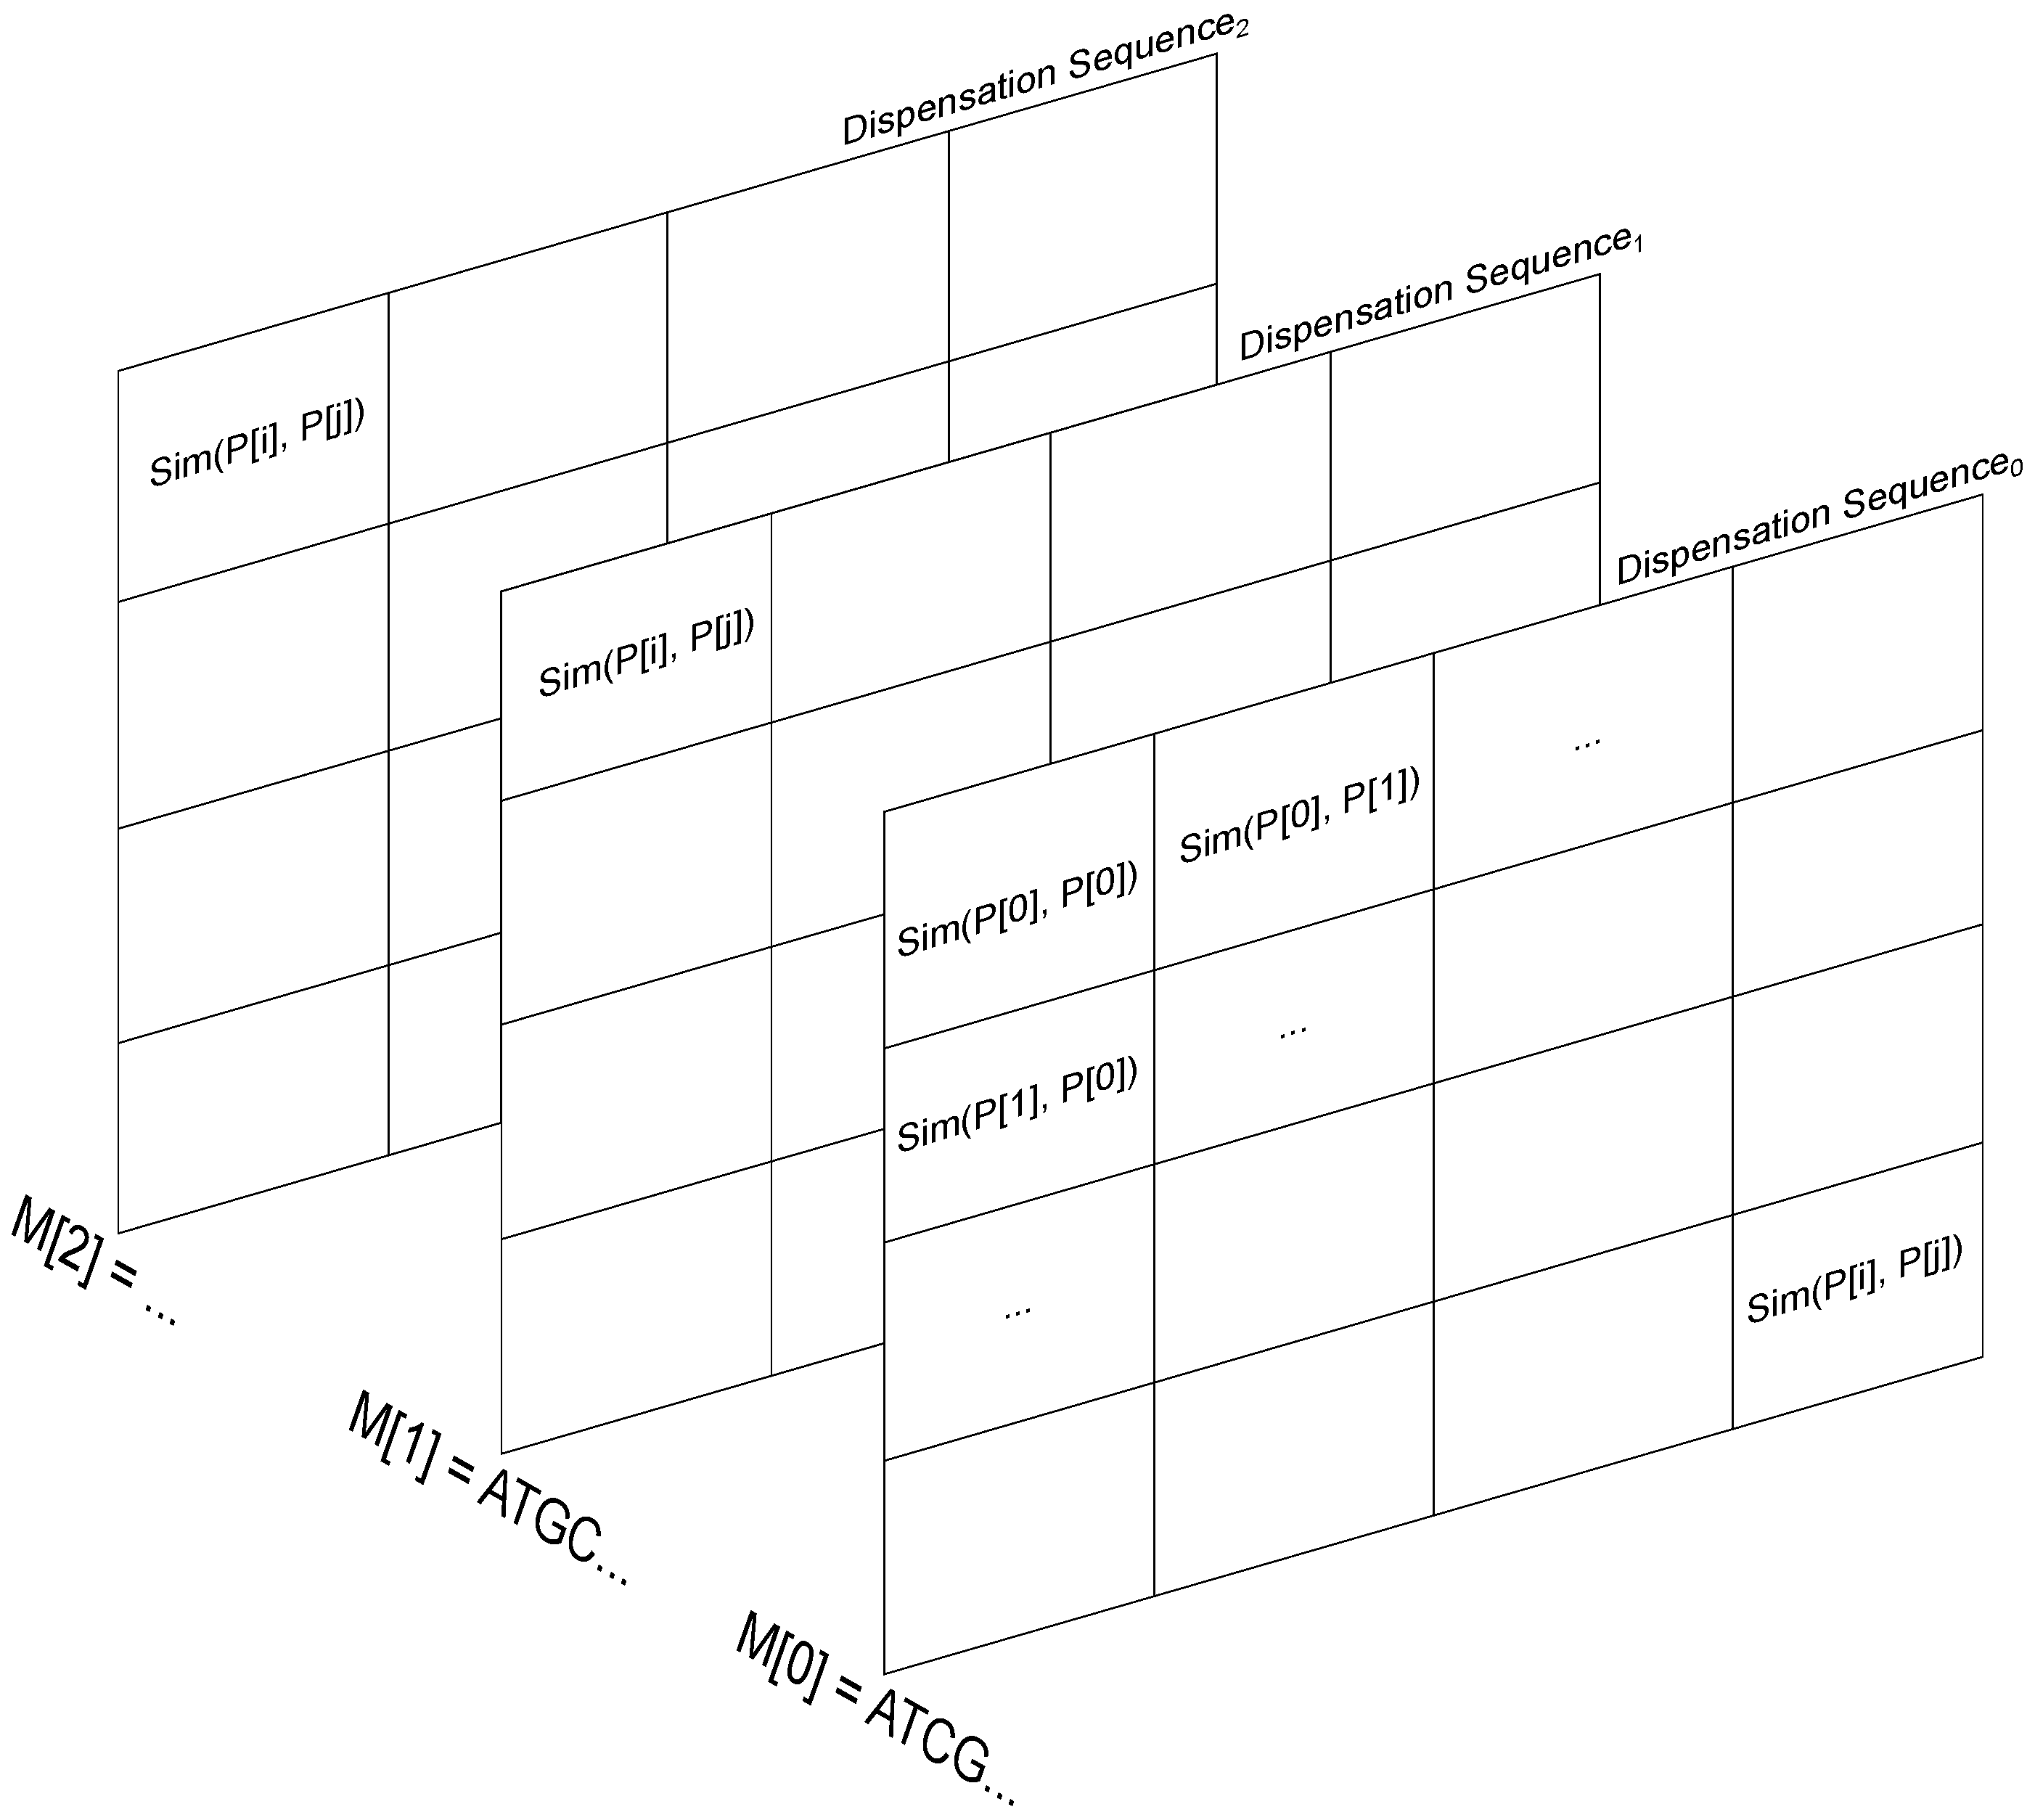
\includegraphics[width=0.7\columnwidth]{graphics/PyroprintSimilarityMatrices.eps}
         \caption{Depiction of the three dimensional matrix $M[n][i][j]$
                  used in CompareSequences($D$, $F$).}
         \label{fig:pyro_matrices}
      \end{figure}

      Each similarity matrix $n \in M[\;]$ is a similarity matrix where the
      $i$th row and the $j$th column contain the Pearson's correlation between
      pyroprints $P[i]$ and $P[j]$ with dispensation sequence $d_n$. This is
      depicted in Figure \ref{fig:pyro_matrices} for clarity. Each pyroprint
      $i \in P[\;]$ is created from the FASTA file $f_m$ where the $i$th
      pyroprint is constructed from the $m$th FASTA file.

      A FASTA file is a file format containing one or many DNA sequences. Each DNA
      sequence (of any length) contained in a FASTA file is preceded by a
      description line beginning with ``\textgreater.'' The description line often includes
      metadata about the following DNA sequence. PyroprintDAT assumes input FASTA
      files contain DNA sequences for each replicate of a particular ITS region.
      For a simple example, using DNA sequences from the 16S--23S ITS region of
      \textit{E. coli}, it is assumed that an input FASTA file contains seven DNA
      sequences as shown in Figure (figure to come). Once the set of pyroprints,
      $P$, contains pyroprints for each FASTA file, $f_m$, a similarity matrix
      $M_k$ is created by comparing each pyroprint $P_i$ against each pyroprint
      $P_j$. The similarity matrix $M_k$ is a symmetric matrix where the each
      position on the diagonal is $1$. Once similarity matrices are computed for
      all candidate sequences, each similarity matrix is assessed based on the
      number of similar/dissimilar pyroprints within the matrix.

      The assessment of the similarity matrices can be done in many ways. One way
      consists of simply minimizing the number of Pearson's correlations that are
      $1$ in the similarity matrix. Another way could be to determine the minimum
      Pearson's correlation values for a percentage of entries in the similarity
      matrix. Yet other ways for assessing the similarity matrix could be to
      determine the average Pearson's correlation, the median Pearson's
      correlation, the lowest sum of all Pearson's correlations, etc.

      \subsection{Dispensation Analysis Results}\label{sec:dat_results}
      %TODO
      $<$TODO$>$

   \section{Interim tool}\label{sec:interim_tool}
      The second tool, simply called pyroAnalysis, was developed in the interim
      period before CPLOP when there was no data management application for
      pyroprints. Data from senior projects and master's theses were managed
      and maintained solely in Microsoft Excel. The goal of pyroAnalysis was to
      provide basic cluster analysis of bacterial isolates and pyroprints
      during this time. Unfortunately, pyroAnalysis had to be built quickly to
      address the immediate needs of Emily Neal's pilot
      study~\cite{Montana:ChronoCluster} and other biology senior
      projects. To speed up the development process, pyroAnalysis accepted
      input as a similarity matrix of Pearson's correlations between pyroprints
      in comma-separated value (CSV) format. Initially, pyroAnalysis only
      provided a proof-of-concept implementation of \textsf{OHClust!} using the
      ontology pictured in Figure \ref{fig:ontology_structure} for Emily Neal's
      pilot study. As data from other pyroprinting senior projects required
      cluster analysis, and Emily Neal expanded her experiments to a six month
      longitudinal, population-based study, the ontology used by
      \textsf{OHClust!} was modified, \textsf{agglomerative clustering} was
      implemented, and other basic features were implemented. Many of the
      features provided by this tool were re-implemented as SPAM (Suite of
      Pyroprint Analysis Methods) and are detailed in Chapter
      \ref{chap:implementation}.

\chapter{OHClust!}\label{chap:algorithm}
   The primary contribution of this thesis is a new clustering technique,
   \textsf{ontological hierarchical clustering} (\textsf{OHClust!}), which was
   designed and developed as a better alternative to \textsf{agglomerative
   clustering}. While \textsf{agglomerative clustering} seems to produce
   meaningful and useful clusters, it is unable to leverage extra information
   associated with pyroprinting studies. \textsf{OHClust!} was developed
   primarily to incorporate pyroprint and isolate meta-data into the clustering
   process. Meta-data is valuable information associated with every collected
   isolate and pyroprint. This includes where and when bacterial isolates were
   collected, whom it was collected by, when it was pyroprinted, the host
   animal from which it was collected, etc. All of this meta-data is unused by
   \textsf{agglomerative clustering}. Unfortunately, it is non-trivial to
   develop a quantitative measure to accommodate isolate and pyroprint
   meta-data in the \textsf{agglomerative clustering} analysis.
   \textsf{OHClust!} is able to leverage meta-data through a hierarchy
   expressed as an ontology. The ontology is then used to guide the order in
   which comparisons are made during clustering.

   \section{Origin and Motivation}\label{sec:origin}
      Originally, Emily Neal used \textsf{agglomerative clustering} to cluster
      bacterial isolates collected during a pilot study of \textit{E. coli}
      populations in the human gut~\cite{Montana:ChronoCluster}. There were two
      issues with \textsf{agglomerative clustering} that motivated the design
      behind \textsf{OHClust!}

      \paragraph{Interpretations} First, the dendograms that
      \textsf{agglomerative clustering} produced from initial clustering runs
      were difficult to interpret because data points had to be manually
      related back to \textit{E. coli} isolates and their meta-data.

      Not only this but the resulting clusters...

      It was determined
      that using some of the knowledge of the experimental structure--swab
      techniques and date of the experiment--could lead to automatically, and
      more accurately, comparing \textit{E. coli} isolates based on their
      meta-data.


      \paragraph{Partitioning} Second, the dendogram showed that there were
      many \textit{E. coli} isolates with very high similarity (Pearson's
      correlation $> 99\%$). Given that \textsf{agglomerative clustering}
      clusters the closest data points first, It was hypothesized that highly
      similar \textit{E. coli} isolates could be partitioned. This could
      improve performance without degrading the quality of the clustering
      results.

      Initially, the objective of \textsf{OHClust!} was to extract useful
      information from a dendogram for a clustering of bacterial isolates. To
      do this, it was necessary to establish some concept of what bacterial
      isolates are more closely related with regards only to meta-data. With
      Emily Neal's pilot study as a reference~\cite{Montana:ChronoCluster}, it
      was established that bacterial isolates collected in the same day would
      be more closely related. Similarly, bacterial isolates collected in
      consecutive days were more closely related than bacterial isolates
      collected several days apart. Finally, bacterial isolates collected using
      swab techniques that were closer to each other temporally were considered
      to be more closely related than bacterial isolates collected at the
      beginning of the day and at the end of the day. The use of meta-data to
      extract more information from the dendogram led to partitioning the data
      based on the meta-data. In this way, it was possible to address
      information extraction and performance in a shared manner.

      The partitions that were explored were representative of the meta-data
      relevant to the population study being conducted. The population study
      consisted of three different methods of sampling \textit{E. coli}
      isolates at regular times during the day--\textnormal{I}mmediate,
      \textnormal{F}ecal, and \textnormal{L}ater. The population study spanned
      14 days. The question being investigated was, ``are there any observable
      patterns of \textit{E. coli} strains and are there any noticeable
      differences in these strains over the two week period?'' The partitioning
      scheme constructed from this meta-data separated \textit{E. coli}
      isolates from different days, and within each day \textit{E. coli}
      isolates were separated based on which sampling method was used for
      collection. The reason for this being the desire to easily interpret
      relationships within subsets of the input dataset--if there is some
      observable \textit{E. coli} strain on any day, does it change between
      days? Further, is there any difference in which \textit{E. coli} strains
      collected \textit{E. coli} isolates belong to depending on the sampling
      method? That is, using different sampling methods, are certain strains of
      \textit{E. coli} more accessible than others. In addition to these
      research questions, there is an intuition that the partitioning scheme
      leveraged, though it was not tested or investigated. That intuition is
      the idea that there is a stronger relationship between \textit{E. coli}
      isolates collected using the same sampling method than those collected
      using different sampling methods. Also, \textit{E. coli} isolates
      collected in the same day have a stronger relationship than those
      collected on different days. The partitioning scheme used by
      \textsf{OHClust!} has since been referred to as an ontological structure,
      which is further described in Section \ref{sec:ontology_structure}. The
      ontological structure has also become a mechanism on which incremental
      updates can be made to \textsf{OHClust!} results.

      Incremental updates can mean several different things as mentioned by
      related work in Chapter \ref{chap:related}. While these many different
      meanings might have converging results, the approach that a clustering
      algorithm takes to incremental updates can vary greatly depending on the
      author's definition of incremental updates. For \textsf{OHClust!},
      incremental updates are discrete sub-datasets that are added to an
      already analyzed, already clustered input dataset. For clarity, Figure
      (figure to come) depicts a dataset that has already been analyzed for
      clusters but there is additional data that wants to be clustered with the
      already clustered dataset. For the work described in this thesis, an
      incremental update is an independent request to cluster data, and not an
      intermediate step in the clustering process. An illustrative example is
      the scenario where data collected during the pilot study described above
      has been clustered and conclusions have been inferred. Then, following
      positive and meaningful results, it is decided that the student wants to
      extend the study and collect data for 14 more days. Instead of taking the
      collective data for all 28 days and clustering it all together, it may be
      desirable to add clusters constructed from the newest 14 days to the
      clusters from the original 14 days. This scenario is depicted in Figure
      (figure to come) and conveys the idea of a single update that doubles the
      size of the original dataset.

      There are two ways in which \textsf{OHClust!} incorporates extra meta-data
      in the clustering process. One way is to organize data points in an
      ontological structure based on specified meta-data of interest. It is
      desirable to detect and analyze patterns and relationships present in
      subsets of the input dataset based on meta-data that is relevant to the
      purpose of the study. \textsf{OHClust!} is able to observe and detect
      patterns in the input dataset in flexible and interesting ways that
      \textsf{agglomerative clustering} is not able to. Because of the way this
      is approached in \textsf{OHClust!}, accuracy of the overall clustering does
      not diverge significantly. Another motivation behind \textsf{OHClust!} is
      improved performance over \textsf{agglomerative clustering}. This performance is
      explored in two aspects: the ability to handle incremental updates and the
      capacity for better parallelization and scalabilty. The extent to which
      \textsf{OHClust!} meets these expectations is investigated in Chapter
      \ref{chap:evaluation}.

   \section{Meta-data and the Ontological Structure}\label{sec:ontology_structure}
      At the core of \textsf{OHClust!}'s design and approach to clustering is an
      ontology based on user-specified meta-data. Before attempting to understand
      how the ontology is constructed and what makes it useful, it is necessary
      to understand what meta-data is. Simply put, meta-data is extra information
      that provides context about data. Examples of meta-data include information
      such as the host species from which collected bacteria originates (if
      known), the day the bacteria was collected, pyroprinted, or stored in the
      database. The difference between meta-data and core data is that meta-data
      describes provenance--information about the origins of an entity--or
      contextual information, whereas core data describes the contents or identity
      of of an entity. Examples of core data include the name of an ITS region and
      the light emittance values of a pyroprint vector. Isolate and pyroprint
      meta-data are especially important for two reasons: it determines the kinds
      of relationships between bacterial isolates that are of interest, and it
      determines whether resulting analysis is biologically meaningful.

      \textsf{OHClust!} was developed around the use of an ontological
      structure for directing the order for clustering. This is unlike
      \textsf{agglomerative clustering} which typically clusters data points in
      descending order of data point similarity. While clustering the most
      similar data points first is a desirable feature, in the context of
      strain differentiation, it is even more desirable to prioritize the
      clustering of data points based on meta-data which provide more
      information regarding the relationships between data points. The
      ontological structure is depicted by Figure \ref{fig:ontology_structure}.
      The ontological structure is represented computationally as a general
      $n$-ary tree as seen in Figure \ref{fig:general_structure}. A tree is a
      type of structure in computer science that is used to organize
      information in a hierarchical manner. An $n$-ary tree is a general type
      of tree such that each level of the hierarchy may have any number $n$
      partitions or sub-hierarchies. The parts of a tree are described as
      follows:
      \begin{description}
         \item[\em{node}] Any item in the ontology, depicted as circles in Figure
                          \ref{fig:general_structure}.
         \item[\em{root}] First node in the tree, located at the top. The only
                          node without a parent.
         \item[\em{leaf}] A bottom-most node in the tree. Any node without
                          children.
         \item[\em{edge}] A connection between any two nodes.
         \item[\em{parent}] In a pair of nodes with a direct connection, the
                            parent node is the top node, or is closer to the
                            root.
         \item[\em{child}] In a pair of nodes with a direct connection, the child
                           node is the bottom node, or is further from the root.
         \item[\em{depth}] The number of edges to get from the root to a
                           particular node.
         \item[\em{level}] Set of all nodes with the same depth.
      \end{description}
      Figure \ref{fig:cluster_structure} shows how a particular ontology with two
      levels may be represented computationally. The root would contain clusters
      of each child node, or sub-hierarchy, the second level of nodes would
      contain isolates separated by month of the study, and the bottom-most level
      of nodes would contain isolates separated by swabbing technique used.

      \begin{figure}[t]
         \centering
         \begin{subfigure}[t]{0.45\textwidth}
            \centering
            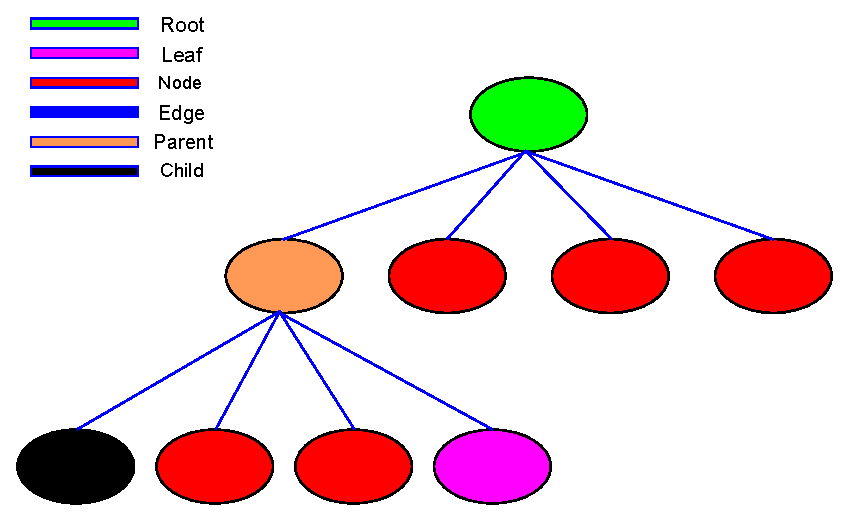
\includegraphics[width=\textwidth]{graphics/IsolateTree.eps}
            \caption{A general structure illustrating the parts of the ontological
                     structure.}
            \label{fig:general_structure}
         \end{subfigure}
         \hfill
         \begin{subfigure}[t]{0.45\textwidth}
            \centering
            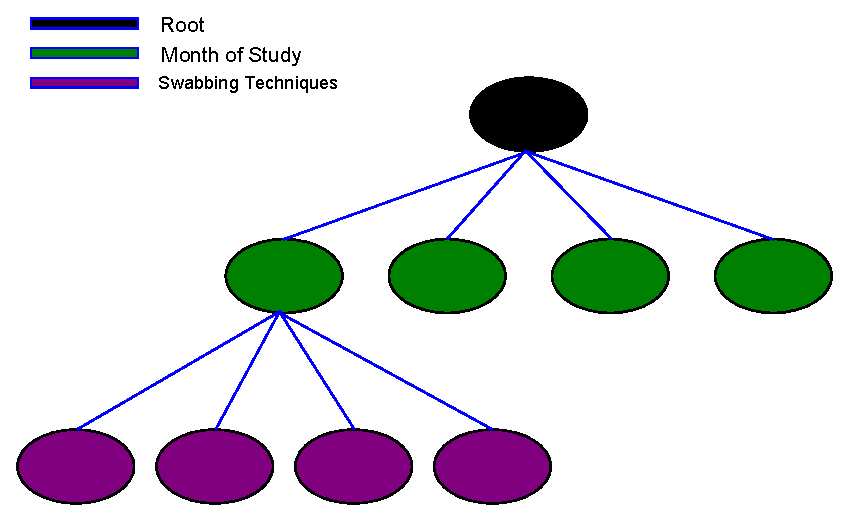
\includegraphics[width=\textwidth]{graphics/IsolateTree_CurrentStudy.eps}
            \caption{The ontological structure for a particular experiment
                     representing the month that the isolates were collected in
                     the first level and the swabbing technique used to collect the
                     isolate in the second level.}
            \label{fig:cluster_structure}
         \end{subfigure}
         \caption{Depictions of a general and particular ontological structure.}
         \label{fig:ontology_structure}
      \end{figure}

      Conceptually, the ontological structure is used in the following manner:
      \begin{itemize}
         \item Isolates are added to the ontological structure starting at the
               root and are passed to appropriate sub-hierarchies.
         \item Clustering takes place bottom-up in the ontological structure,
               starting at the leaves.
         \item Within each node data is clustered using \textsf{agglomerative
               clustering}
         \item When data in a node is finished being clustered, the resulting
               clusters are propagated up the tree, and the process repeates.
         \item Optionally, the user may specify whether to incrementally grow
               clusters or to integrate all clusters together at once at any
               internal node.
      \end{itemize}
      The pseudocode for \textsf{OHClust!} and how it uses the ontological structure is
      described in Section \ref{sec:ohclust}.

   \section{Data Transformation}
      \textsf{OHClust!} uses a \textit{thresholded version} of the Pearson
      correlation coefficient to compare individual pyroprints to each other.
      Ideally, when comparing pyroprints, the similarity falls into three
      categories: similar, squishy, dissimilar. The thresholded version of
      Pearson's correlation takes this into account by transforming
      similarities above the $\alpha$ threshold to $1$ and similarities below
      the $\beta$ threshold to $0$, as shown here:
      $$
         thr(sim(I_{a}, I_{b})) = \begin{cases}
                              0 & if sim(I_{a}, I_{b}) < \beta \\
                              1 & if sim(I_{a}, I_{b}) > \alpha \\
                              sim(I_{a}, I_{b}) & otherwise \\
                              \end{cases}
      $$
      This transformation is the mechanism for ensuring strongly connected
      isolates at the core of each cluster.


      In order to appropriately interpret the computed correlation coefficient
      between a pair of pyroprints, we utilize a pair of threshold values
      $\alpha$, the \textit{upper threshold}, and $\beta$, the \textit{lower
      threshold}\footnote{Default values are $\alpha = .995$ and $\beta =
      .99$}.

   \section{OHClust! Algorithm}\label{sec:ohclust}
      There are three primary components of the \textsf{OHClust!} algorithm:
      \begin{enumerate}
         \item parse and populate ontological structure
         \item organize data into ontological structure
         \item iterate over the ontological structure and cluster data
               beginning at the leaves until final clusters are percolated to
               the root.
      \end{enumerate}

      The contents, or features, layout, and ordering of the ontological
      structure is user-specified. Ideally, ontology specification is done via
      a graphical tool. However, ontology specification is currently supported
      through an intermediate format of the form:
      \begin{verbatim}
         <table>.<attribute>(<option, ...>):<attribute value, ...>;
         <table>.<attribute>(<option, ...>):<attribute value, ...>;
         ...
      \end{verbatim}
      The ontological structure is built top down such that each line
      corresponds to a level of the ontological structure. The \textit{table}
      and \textit{attribute} values are to ensure access to the correct data in
      a database. The \textit{option} value represents possible options for
      clustering at each internal node. Some example options are
      \textit{TimeSensitive}, \textit{SimilarCorr}, and \textit{SquishyCorr}.
      The TimeSensitive option forces an ontological node to cluster data
      from its children in-order as data is percolated up. If this option is
      not specified, then an ontological node will acquire data percolated from
      each of its children then cluster all of the percolated data as a single
      dataset. The SimilarCorr option forces ontological nodes to cluster data
      using the upper threshold, $\alpha$, before percolating data upwards.
      Alternatively, the SquishyCorr option forces ontological nodes to cluster
      data using the lower threshold, $\beta$, before percolating data upwards.
      Important to note, ontological node options are set on a level by level
      basis. Meaning, each ontological node on the same level of the
      ontological structure have the same options set. This is partially for
      ease of implementation, but mostly because setting different options for
      various ontological nodes on the same ontological level makes little
      sense.

      The organization of data points into the ontological structure is done
      quite easily. It is as simple as keeping track of meta-data for each data
      point and then passing each data point to the corresponding child node in
      the ontological structure. Each data point is initially stored in the
      leaf nodes of the ontological structure. Once clusters are formed from
      the data contained in an ontological node they are percolated up the
      tree.

      Iteration over the ontological structure to execute clustering is seen in
      the pseudocode provided below:
      \begin{algorithmic}
         \Function {ontologicalCluster}{$D$, $N$}
            \State $C \gets \emptyset$

            \If {$N = null$}
               \Comment{If node is null; return emptyset}
               \Return $C$
            \EndIf

            \If {isSimilarCorr($N$)}
               \Comment{If node has SimilarCorr option}
               \State $T \gets \alpha$
            \Else
               \If{isSquishyCorr($N$)}
                  \Comment{If node has SquishyCorr option}
                  \State $T \gets \beta$
               \EndIf
            \EndIf

            \If {$|$children($N$)$| > 0$}
               \Comment{If node has children; cluster each child}
               \For {$n_i \in$ children($N$)}
                  \State $C \gets C\;\cup$ ontologicalCluster($D$, $n_i$)

                   \If {isTimeSensitive($N$)}
                     \State $C \gets C\;\cup$ agglomerativeCluster($D$, $C$, $T$)
                  \EndIf
               \EndFor

               \If {!isTimeSensitive($N$)}
                  \State $C \gets C\;\cup$ agglomerativeCluster($D$, $C$, $T$)
               \EndIf

            \Else
               \Comment{If leaf node; cluster data}
               \State $C \gets$ agglomerativeCluster($D$, $C$, $T$)
            \EndIf

            \Return $C$
         \EndFunction

         \Function {agglomerativeCluster}{$D$, $C$, $T$}
            \State $C' \gets C$
            \State ($c_{a}$, $c_{b}$) $\gets \emptyset$
            \State $D[\;] \gets$ computeSimilarities($D$, $C'$)

            \While {$|C'| > 1$}
               \State ($c_a$, $c_b$) $\gets$ \textit{arg}max($D[\;]$)

               \If {sim($c_a$, $c_b$) $\ge T$}
                  \State $C' \gets C'\;- c_{a}$
                  \State $C' \gets C'\;- c_{b}$

                  \State $C' \gets C'\;\cup$ combineClusters($c_a$, $c_b$)

                  \State $D[\;] \gets$ computeSimilarities($D$, $C'$)
               \EndIf
            \EndWhile

            \Return $C'$
         \EndFunction

         \Function {computeSimilarities}{$D$, $C$}
            \For {$c_j$, $c_k \in C$}
               \State $D[j, k] \gets$ sim($c_j$, $c_k$)

               \If {$D[j, k] \ge \alpha$}
                  \State $D[j, k] \gets 1$
               \ElsIf {$D[j, k] < \beta$}
                  \State $D[j, k] \gets 0$
               \EndIf
            \EndFor

            \Return $D$
         \EndFunction
      \end{algorithmic}
      For this pseudocode, the \textsf{computeSimilarities} and
      \textsf{agglomerativeCluster} functions are straightforward and do all of
      the major work. All similarities between clusters are calculated by
      \textsf{computeSimilarities} and stored in the similarity matrix $D$. The
      function \textsf{agglomerativeCluster} is the \textsf{agglomerative
      clustering} algorithm and produces clusters given a dataset.

      While \textsf{computeSimilarities} and \textsf{agglomerativeCluster} are
      the primary working functions, \textsf{ontologicalCluster} handles
      iteration over the ontological structure and cluster percolation between
      ontological nodes. It is a recursive function, where the first call is
      passed the root of the ontological structure as $N$. For each child node
      of $N$, the function is called again, passing the child node as $N$ for
      the recursive function call. Once a leaf node is reached, the data stored
      in the leaf node is clustered as described in
      \textsf{agglomerativeCluster} using a threshold value. The threshold value
      used is determined by options set for the ontological node by the user.
      If the ontological node has the SquishyCorr option set, then the lower
      threshold, $\beta$, is used. If the SimilarCorr option is set, then the
      upper threshold, $\alpha$, is used. The clustering returned by
      \textsf{agglomerativeCluster} is then passed to the parent of $N$, the
      current ontological node. Once all child nodes of an ontological node has
      been clustered, then the ontological node itself may be clustered. In
      this way, data is initially stored in leaf nodes. Once clustering is
      invoked, data is clustered at the bottom level, and results are
      percolated up through the cluster.

   \section{Algorithmic Analysis}\label{sec:algorithm_analysis}
      In this section, the algorithimic complexity of \textsf{OHClust!} is
      analyzed. For this analysis, only the complexity of steps directly
      pertinent to cluster analysis are considered. This includes:
      \begin{itemize}
         \item Placing data points appropriately in the ontological structure
         \item Traversing the ontological structure, applying agglomerative
               clustering to data in each node and percolating resulting
               clusters up the structure.
      \end{itemize}
      For our analysis we consider the following notation: Let $n$ be the
      number of isolates being clustered, let $p$ be the number of partitions,
      or children, that a node in the ontology has, and let $k$ be the depth of
      the ontology. Note that each level $k$ of the ontology will have the same
      number of partitions $p$ for each node, but the number of partitions may,
      and typically will, differ between levels $0, \ldots, k$. For the
      analysis given here, we assume a fixed $p$ as the maximum $p$ for any
      given $k$.

      As the first step of \textsf{OHClust!} we place each isolate into the
      ontological structure. The ontology is always constructed as a full,
      balanced tree. That is, the ontology has $p^{k}$ leaves and $p^{k} - 1$
      internal nodes. In the best case, $n$ isolates are evenliy distributed
      across $p^{k}$ partitions. In the worst case, all $n$ isolates are placed
      in a single partition. In either case, isolates are percolated down the
      ontology with the same time complexity. At each level $k$ there are $p$
      options and isolates will percolate down $k$ levels on average, assuming
      a general ontology. This requires $pk$ comparisons or
      considerations before an isolate arrives at its appropriate location in
      the ontology. For $n$ isolates this yeilds a time complexity of $npk$. As
      $k$ is a small number on average ($k=2$ for Emily Neal's pilot study and
      deep study, and $k \in \{2, 3\}$ for tests in Chapter
      \ref{chap:evaluation}), and $p$ is a small number relative to $n$, the
      complexity for inserting isolates into the ontology is considered
      $O(n)$.

      The second step of \textsf{OHClust!} can, itself, be broken into two
      smaller steps:
      \begin{itemize}
         \item \textsf{agglomerative clustering}
         \item traversing and percolating clusters through the ontology.
      \end{itemize}
      At each node, \textsf{OHClust!} applies a clustering algorithm. In this
      thesis, \textsf{agglomerative clustering} is applied. Although a best
      case partitioning of isolates is $\frac{n}{p^{k}}$ per leaf, we first
      consider a worst case scenario of $n$ isolates at a single leaf. In this
      case, the complexity is exactly the same as agglomerative clustering.
      That is, there are $n$ clusters to be considered, and there are
      $\frac{n\;(n-1)}{2}$ comparisons to be made before two clusters can
      be joined. This is approximately $O(n^2)$ for each iteration of
      \textsf{agglomerative clustering}. As two clusters are joined on each
      iteration until no more clusters can be joined, this yields a worst case
      of $n-1$ iterations. For $n$ isolates in a single leaf of the ontology,
      and for \textsf{agglomerative clustering} in general, we observe a time
      complexity of $O(\frac{n\;(n - 1)}{2} \times (n - 1))$ or, simply
      $O(n^{3})$.

      Consider the best case, which approximates the average case, such that
      there are $\frac{n}{p^{k}}$ isolates located at each leaf. Taking
      similar steps as before, we consider the complexity of applying
      \textsf{agglomerative clustering} at a node, except for $\frac{n}{p^{k}}$
      isolates instead of $n$. Predictably, we observe a complexity of
      $O(\frac{n}{p^{k}}\;(\frac{(\frac{n}{p^{k}} - 1)}{2} \times
      (\frac{n}{p^{k}} - 1))$. Again, considering that $k$ is on average a
      small number and that $p$ is typically small in comparison to $n$, this
      complexity is asymptotically upper bounded by $O(n^{3})$.

      As \textsf{OHClust!} must percolate cluster results from each node up the
      trree, we note that $O(n^{3})$ is the base case time complexity for
      clustering at a leaf. We then consider the following recurrence relation
      for \textsf{OHClust!}:
      $$
         T(n) = \begin{cases}
                  \Theta(1) & if n < c,\\
                  pT(n/p) + O(n^{3}) & otherwise.\\
                \end{cases}
      $$
      For a leaf that has $n <$ some small constant $c$ isolates, the
      complexity is considered constant. Otherwise, consider a node $n_{m}$
      where $m$ is the number of levels that have completed clustering. For
      example, $m=0$ when clustering data located in the leaves of the
      ontology, and $m=1$ when clustering takes place at the level above $k$.
      A given node in the ontology, during clustering, must wait for each
      $p_{i} \in p$ child to cluster a subset of the data. If considered from
      the perspective of $n_{m}$, the parent node of $p_{i}$, in the average
      case, then each child $p_{i}$ must cluster $\frac{1}{p}$ of the data, or
      $\frac{n}{p^{k-m}}$ data for the $m$th level. Once clustering has
      completed at the $m - 1$ level, then clustering at node $n_{m}$ takes
      $O(n^{3})$ where $n$ is actually $\frac{1}{p}$ of the data to be
      clustered for level $m + 1$. Note that $T(n)$ need not
      consider the time to partition data into sub problems for each child
      $p_{i}$ of $n_{m}$, because that is accounted for during the first step
      of \textsf{OHClust!} where isolates are placed in the ontology. A
      recursion tree for this recurrence relation is shown in Figure
      \ref{fig:recursion_tree}. Notice that unlike typical $n$-ary trees, the
      ontological structure used by \textsf{OHClust!} has constant depth $k$
      instead of variable length $n\log n$.

      \begin{figure}[t]
         \centering
         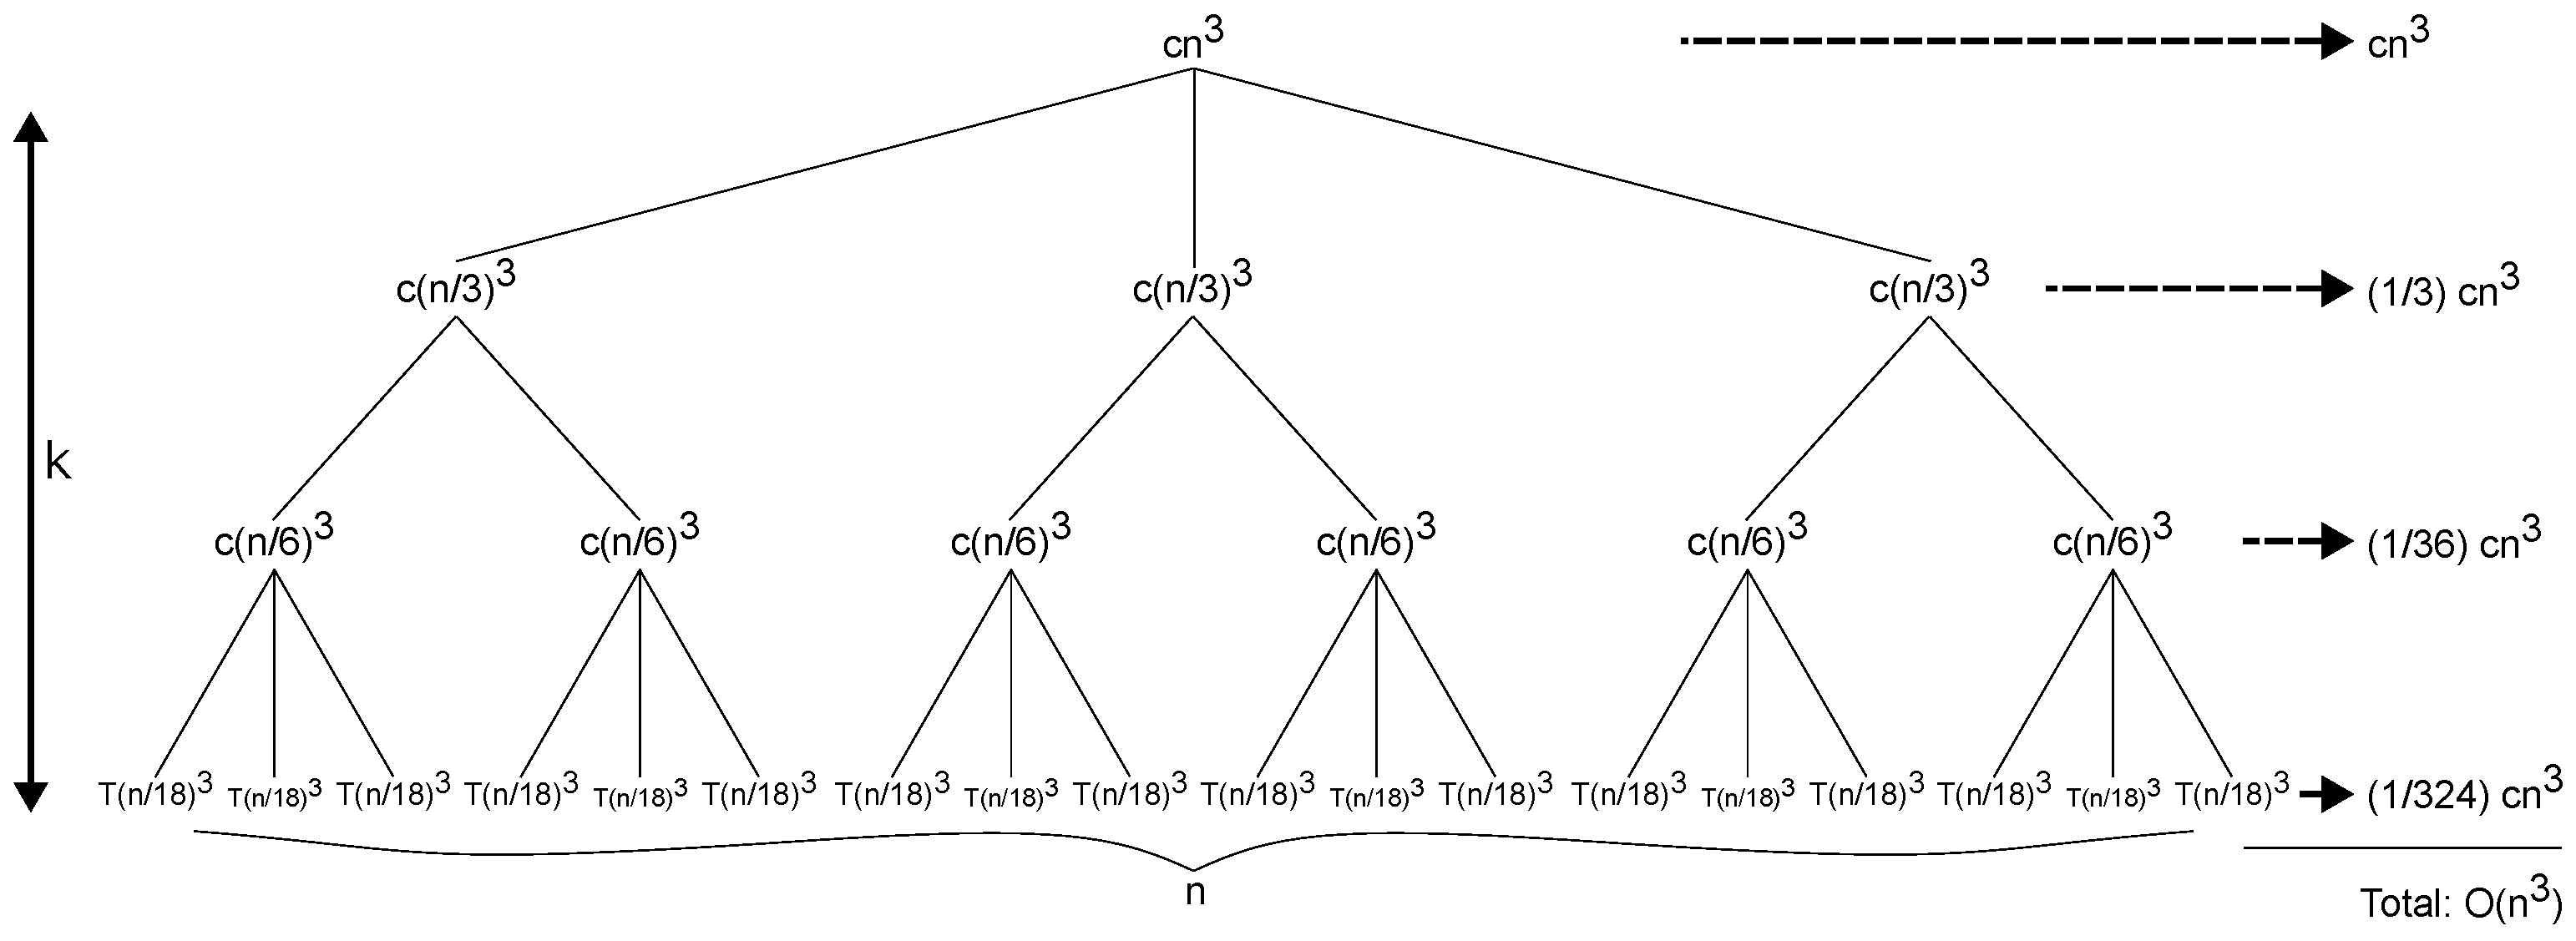
\includegraphics[width=\textwidth]{graphics/recursion_tree.eps}
         \caption{An example of the complexity for clustering in
                  \textsf{OHClust!}}
         \label{fig:recursion_tree}
      \end{figure}

\chapter{Related Work}\label{chap:related}
   \section{Incremental Clustering}\label{sec:incr_cluster}
   Since \textsf{OHClust!} is claimed to be applicable to data types other than
   biological, this section discusses incremental clustering algorithms
   developed for generic datasets. These algorithms were developed to
   incrementally cluster data streams or datasets too large to fit in main
   memory. While this definition of incremental clustering is still applicable
   and relevant to our notion of incremental clustering, there are some
   assumptions that may cause divergence between the optimal clustering of a
   growing dataset and proposed clustering of these algorithms. More
   specifically, clustering a dataset in increments, still has the assumptions
   of a single, whole dataset. In contrast, clustering a dataset that is
   updated in increments has the assumptions that the ideal number of clusters
   may change between updates. The subtle difference may make a difference in
   how quickly produced clusters diverge from optimal clusters, and thus affect
   how frequently the accumulated dataset must be re-clustered.

   %BIRCH description%
   BIRCH, Balanced Iterative Reducing and Clustering using Hierarchies, is a
   clustering method developed by Zhang, et al. to address the problem of
   clustering large datasets and minimizing I/O costs~\cite{Zhang:BIRCH}. BIRCH
   incrementally clusters numerical data by doing a scan of the target dataset
   until memory constraints are reached. Each chunk of data is added to an
   N-ary tree, called a cluster feature (CF) tree, which represents clusters as
   internal nodes and maintains only aggregate information for each cluster.
   The aggregate information, and clustering requirements, are computed based
   on basic algebraic functions: Each data point is represented as a triple of
   the form $D = (N, LS, SS)$ where a data point $D$ is assumed to be a vector,
   $N$ is the number of dimensions, $LS$ is the linear sum of the dimensions of
   $D$, and $SS$ is the squared sum of the dimensions of $D$. In this way,
   distances (not similarities) are additive and easily computed in a single
   scan of the data. This approach uses the CF Tree as a fast, guiding method
   for directing a data point to the appropriate cluster. However, determining
   an appropriate, meaningful CF representation is difficult at best.

   %Fast and Stable Incremental Clustering description%
   Young, et al.'s work on incremental clustering takes a partitional approach
   to clustering~\cite{Young:Incremental}. The described work utilizes a
   competitive learning algorithm that adjusts itself based on a calculated
   pseudo-entropy of the clusters such that a tradeoff is made between updating
   centroids aggressively earlier in the clustering process (earlier iterations
   and/or updates) and updating centroids conservatively later to ensure
   cluster stability. Additionally, there is a credit-based algorithm for
   preventing centroid starvation which is computed based on a fixed value or
   the previously calculated pseudo-entropy such that centroids selected for
   updates lose credit and centroids that are starving accumulate credit over
   time. Although Young, et al. mention the importance of being mindful of the
   possibility that clusters may move, disappear, or reappear, the described
   work only discusses moving centroids and assumes a fixed number of
   centroids. Since the number of clusters that may be formed from clustering
   pyroprints is completely unknown, and will grow unpredictably as more data
   is gathered from different regions, a partitional scheme with a fixed number
   of centroids is not very applicable.

   \section{Incremental Clustering for 16S rRNA Sequences}\label{sec:seq_incr_cluster}
   This section discusses incremental clustering algorithms that were
   developed specifically for clustering DNA sequence reads. These are
   especially relevant to the work described in this thesis as \textsf{OHClust!} was
   developed with pyroprints in mind. Incremental clustering algorithms
   described in this section are all derived from a greedy incremental sequence
   clustering algorithm, hereafter referred to as \textit{SeqClustering} for
   brevity, developed in 1998 by Holm and Sander~\cite{Holm:Greedy}. The
   motivation for this incremental clustering algorithm was to effectively
   handle continuously growing biological datasets, specifically protein
   sequences, and to efficiently determine and convey clusters of similar
   protein sequences. Due to the high volume of redundant protein sequence
   reads, Holm and Sander decided that each cluster should be represented by a
   single data point, or sequence read. By using a representative data point
   for each cluster, it was much more efficient to compute cluster membership
   for each unclustered data point and to convey meaningful, non-redundant
   information for understanding each cluster. Variants of this clustering
   algorithm refer to the representative sequence read of a cluster as a
   \textit{seed}. This algorithm, as well as its variants such as
   CD-HIT~\cite{Li:CD_Hit}, UCLUST~\cite{Edgar:UCLUST}, and
   DySC~\cite{Zheng:DySC}, cluster DNA sequences by using a single sequence as
   a cluster representative to which unclustered DNA sequences are aligned
   against. That is, DNA sequences are data points, and each cluster is
   represented by a single data point, against which other data points are
   compared. The comparison metric used is typically a sequence alignment,
   which gives a similarity score based on the edit distance between the
   compared sequences.

   One variant of Holm and Sander's SeqClustering algorithm is cd-hit and each
   of its variants: cd-hit-2d, cd-hit-est, cd-hit-est-2d~\cite{Li:CD_Hit,
   Li:Redundancy}. Cd-hit has SeqClustering as its core algorithm, but
   optimizes performance by using short word filtering instead of sequence
   alignments as its comparison metric. Short word filtering, in short,
   verifies that the compared sequences share a minimum number of identical
   short substrings, referred to as `words', such as dipeptides, tripeptides,
   etc. For certain length words, it's possible to have indices of the seed for
   a cluster so that it is very fast to compare a sequence to the seed via
   short word filtering.

   %DySC Greedy Clustering Description%
   Another, very relevant, variant of the SeqClustering algorithm, called
   dynamic seed clustering (DySC), was developed by Zheng, et
   al.~\cite{Zheng:DySC}. DySC is a clustering algorithm developed for reads of
   the 16S rRNA marker gene commonly used in microbial studies. DySC
   differentiates itself from other SeqClustering algorithms by using both
   fixed seeds and dynamic seeds. Seeds in SeqClustering correspond to a fixed
   seed in DySC, whereas SeqClustering has no equivalent to dynamic seeds in
   DySC. Using dynamic seeds, DySC constructs \textit{pending clusters},
   clusters containing reads that are not within a similarity threshold to the
   fixed seeds. Pending clusters are transient and will either join a fixed
   seed cluster or become a fixed seed cluster after reaching a specified size.
   Zheng, et al. claim that DySC is able to improve cluster quality while
   maintaining comparable runtime compared to UCLUST and
   CD-HIT~\cite{Zheng:DySC}.

   %Incremental Clustering Description%
   Yooseph, et al. have done work on the incremental clustering of microbial
   metagenomic sequence data~\cite{Yooseph:Incremental}. Incremental clustering
   is a three stage clustering process based on CD-HIT. \textbf{First Stage}.
   patterns are combined with clusters in three steps, each with 90\%, 75\%,
   and 60\% identity thresholds, respectively. Incremental clustering takes
   this approach of decreasing identity thresholds for efficiency and quality.
   For efficiency, cd-hit-2d runs faster at high thresholds (90\%) than at low
   thresholds (60\%). For quality, the parallel implementation of cd-hit-2d
   being used by Yooseph, et al. at the time (2008) could only assign patterns
   to the first cluster whose similarity met the threshold. \textbf{Second
   Stage}. Patterns from the data set not incorporated into clusters in stage
   one are clustered together using cd-hit at 90\%, 75\%, and 60\% identity.
   The clusters formed here are referred to as \textit{core clusters} by
   Yooseph, et al. \textbf{Third Stage}. Two similarity measures are used to
   join \textit{big core clusters} (cluster with cardinality $\ge$ 20) with
   each other and small core clusters or singleton clusters (cluster with
   cardinality $=$ 1) with final clusters, respectively FFAS and PSI-BLAST.

   %Relate algorithms to work%
   Each variant of the SeqClustering algorithm is highly relevant to \textsf{OHClust!}
   in their ability to cluster data incrementally and their relevance to
   biological data. Using a seed, or cluster representative, that is $\le 90\%$
   similar to all other seeds allows new clusters to easily form, which is
   important to consider for a continuously growing dataset. Interestingly,
   Yooseph, et al.'s work on incremental clustering and its three phase
   approach seems to be the most similar to \textsf{OHClust!}. Where Yooseph, et al.
   takes a three phase approach, \textsf{OHClust!} seeks to improve clustering
   performance and quality in a two phase approach. The first phase creates
   core clusters using the $\alpha$ threshold, and the second phase
   incorporates pyroprints into a boundary or fuzzy cluster using the $\beta$
   threshold. However, incremental clustering partitions its data in a three
   tier scheme by thresholds (90\%, 75\%, and 60\%) instead of the hierarchical
   partitioning employed by \textsf{OHClust!}.

   Seemingly, these algorithms are more accommodating of updates than
   incremental clustering in Section \ref{sec:incr_cluster} and can handle
   situations where constructed clusters may significantly differ from initial
   predictions of observable patterns. In this way, these algorithms may be
   more amenable to incremental clustering across updates than \textsf{OHClust!}.
   However, there is a major aspect in which SeqClustering algorithms differ
   from \textsf{OHClust!}: the use of a core cluster in \textsf{OHClust!} instead of a
   representative data point. Instead of a representative data point, the use
   of core clusters potentially reduces clustering errors of pyroprints,
   especially across updates. This is especially important since pyroprints are
   not exactly DNA sequences and are vulnerable to machine and human error.
   Additionally, cluster similarity is computed using each point in the cluster
   (in the case of average-link or ward's method) instead of a single
   comparison. Due to this being computationally more expensive, the advantages
   and disadvantages of not using cluster representatives are explored in
   Chapter \ref{chap:evaluation}.

\chapter{Suite of Pyroprint Analysis Methods}\label{chap:implementation}
   The implementation of Suite of Pyroprint Analysis Methods (\textit{SPAM})
   described in this chapter was done in Java, and compliant with Java 1.6. The
   majority of users have JRE 1.6 installed, but not JRE 1.7. Additionally, the
   code is accessible from the SPAM repository on
   Github\footnote{http://www.github.com/drin/spam}. This framework is written
   such that many components can be written consistently and interchangeably,
   including clustering algorithms, comparison metrics, and data types. In
   Section \ref{sec:design} the overall design of the framework is described,
   while Sections \ref{sec:data_types} and \ref{sec:metrics} discuss how data
   types can be written, and how comparison metrics are called and can be
   implemented, respectively. Finally, Section \ref{sec:analysis} details how
   analysis algorithms--particularly hierarchical clustering algorithms--can be
   extended and customized. This chapter also has a dual purpose of describing
   how the algorithm has been implemented, and providing a reference of
   documention for anyone desiring to use or extend the code provided.

   Although discussed further in Chapter \ref{chap:evaluation}, it is
   worthwhile to note here that this implementation was not used for larger
   test sets in evaluation. However, the implementation of SPAM described here
   is currently able to perform well enough for current dataset sizes.
   Unfortunately, there is still a lot of work to be done on this framework in
   order to achieve good performance yet maintain modularity and flexibility.

   \section{Design}\label{sec:design}
      SPAM was designed to be a maintanable, modular framework for analyzing
      pyroprints. The design of SPAM heavily emphasizes the use of objects and
      polymorphism to achieve these goals. Specifically, there are four
      components of pyroprint analysis that this framework aims to make easy
      and accessible to any developer working with pyroprints:
      \begin{itemize}
         \item Custom data types
         \item Comparison metrics
         \item Analysis methods
      \end{itemize}
      Bacterial isolates, ITS regions, and pyroprints are represented in SPAM
      using custom data types. While pyroprint analysis will usually not need
      any other custom data types, as pyroprint analysis is applied to other
      FIB or other environments, it may be something of interest in the future.
      At the very least, the design of SPAM to flexibly accommodate custom data
      types allows SPAM to be applied to many different types of data. It is
      incredibly important for comparison metrics to be modular and flexible.
      Pyroprinting is a technique that is still very new. As other aspects of
      pyroprints are considered, for example peak width or peak area, the
      application of other comparison metrics will be desirable or studied.
      Also, the use of different analysis methods is also important. It is
      possible that partitional clustering algorithms, when explored, will be
      capable of producing similar accuracy of bacterial strain identification
      more quickly. It may also be possible that other variants of hierarchical
      clustering developed elsewhere may prove to be more useful or applicable
      to pyroprints than \textsf{OHClust!} It is important that this pyroprint
      analysis framework be easily modified to incorporate new and interesting
      methods to encourage further research with pyroprints at a minimal cost.

   \section{Data Types}\label{sec:data_types}
      Custom data types are necessary and allow SPAM to be applied to datasets
      other than pyroprinting, but also allows for a great amount of
      flexibility in the aspects of pyroprinting that can be researched and
      investigated. Custom data types are expected to extend the
      \textit{Clusterable} abstract class. This class is simple, and all
      necessary information for clustering can be accessed through this
      interface. In this way, clustering modules can be written and used
      without worrying about specifics of the data types involved in
      clustering. The Clusterable class has a name attribute, \textit{mName},
      which serves as the basis of identity and equality, and maintains a
      collection of data points, \textit{mData}, which serves as the basis of
      content. While it is common to use simple data types or numeric data
      types during clustering, SPAM was developed around pyroprints and
      bacterial isolates, which are complex data types consisting of extra
      associated data points. Additionally, the Clusterable class has a
      \textsf{compareTo} method that should be overridden with a data type
      specific implementation of how comparisons are made. Otherwise, the
      Clusterable class provides some convenience methods for accessing mData
      and mName.

      An important custom data type other than Clusterable is the abstract
      class, Cluster, which provides the basic implementation of a
      Cluster. The Cluster class consists of meta-data labels, \textit{mLabel},
      a cluster similarity function, \textit{mMetric}, a corresponding
      dendogram, \textit{mDendogram}, a set of elements contained in the
      cluster, \textit{mElements}, and some extra cluster information.
      Generally, a cluster is a simple data structure that contains similar
      data points, and can be compared with other clusters.

      Important to the general analysis of pyroprinting, there are three custom
      data types located in the \textit{biology} package. These data types are
      \textit{Isolate}, \textit{ITSRegion}, and \textit{Pyroprint},
      corresponding to bacterial isolates, ITS regions, and pyroprints,
      respectively. Each of these data types are simply implemented, primarily
      containing a name (the identifier of the data type, i.e. ``Hu-123'' for a
      human and a unique integer ID for pyroprints), associated data, and a
      comparison method. Each data type is implemented in a way that reflects
      the relationship between the three components. An isolate maintains in
      its collection, mData, a set of ITS regions (Set<ITSRegion>). Practically
      speaking there are only two ITS regions in use, 16S--23S and 23S--5S,
      however, a set of ITS regions allows for flexibility in the future to
      expand to several ITS regions. An ITS region maintains in its collection,
      mData, a set of pyroprints. Each pyroprint maintained in the collection
      of an ITS region is a pyroprint that was constructed from that ITS region
      of a particular isolate. For example, an isolate, $I_{a}$, has a set of ITS
      regions, $R^{a} = \{16-23, 23-5\}$. The region $R_{16-23}^{a} = \{P_1,
      \ldots, P_k\}$ contains $k$ pyroprints constructed from the 16S--23S ITS
      region of Isolate $I_{a}$. Unfortunately, the descriptiveness and
      richness of the relationships represented in this way complicate the
      transformation from a relational database representation of bacterial
      isolates and pyroprints and performance is lost. On the other hand, the
      custom data types accurately represent the data and relationships within
      the data.

   \section{Comparison Metrics}\label{sec:metrics}
      Various comparison metrics have only vaguely been investigated, and
      alternate comparison metrics are not well understood. For future
      research, several comparison metrics will need to be experimented with
      and researched for pyroprinting. To define a custom comparison metrics,
      the abstract class, \textit{DataMetric}, should be extended.

      DataMetric was designed to be relevant to any possible kind of comparison
      metric. DataMetric maintains state in a result value, \textit{mResult},
      and error state in an integer, \textit{mErrCode}. Accessible methods are
      \textsf{reset}, which sets mResult to a default value, \textsf{apply},
      which defines how the comparison metric is implemented, \textsf{result},
      which simply returns mResult, and various methods for accessing or
      setting mErrCode. For many basic comparison metrics, it is possible to
      override only the \textsf{apply} method and the DataMetric class will be
      functional.

      To help manage the various levels of comparison required when analyzing
      bacterial isolates, the DataMetric class uses java generics to
      define the data type it compares. For example, a DataMetric that compares
      isolates is defined as DataMetric<Isolate>, DataMetric<ITSRegion> for a
      DataMetric that compares ITS regions, and so on. This is to help the
      developer ensure that the correct DataMetric is being used for the
      correct data types. Additionally, comparison metrics maintain state so
      that it is simple to implement a similarity function like Pearson's
      correlation using the DataMetric class in a way that is flexible and
      robust.

   \section{Analysis Methods}\label{sec:analysis}
      All clustering analysis methods are expected to implement the
      \textit{Clusterer} interface, making necessary clustering actions
      generally available: \textsf{getClusters} and \textsf{clusterData}.
      However, most cluster analysis methods will not implement Clusterer
      directly, the only cluster analysis methods that directly implement the
      clusterer interface include: PartitionalClusterer and
      HierarchicalClusterer. These methods abstractly define partitional
      clustering algorithms and hierarchical clustering algorithms,
      respectively. Currently, HierarchicalClusterer is the only one
      implemented, though PartitionalClusterer will need to be implemented when
      a partitional clustering algorithm, such as \textit{k-means}, is
      integrated into SPAM. The class inheritance hierarchy for OHClusterer,
      the class that implements \textit{OHClust!}, currently includes:
      \begin{itemize}
         \item Clusterer (interface)
         \item HierarchicalClusterer (abstract class)
         \item AgglomerativeClusterer (class)
         \item OHClusterer (class)
      \end{itemize}

      Clusterer defines the method \textsf{clusterData}, which provides and defines a
      standard point of access to invoking any clustering algorithm's
      clustering. The \textsf{clusterData} method simply takes as input
      a list of clusters to analyze. This is so that Clusterer objects do not
      need to be constructed with a dataset of clusters, which would encourage
      a new object be made for each clustering run. Additionally, although it
      cannot be enforced by the Clusterer interface, cluster analysis methods
      should be constructed with appropriate threshold values. With this
      approach, the \textsf{clusterData} method does not require threshold
      values as input, but can still construct and maintain clusters
      appropriately. For variants of hierarchical clustering algorithms that
      use different threshold values (e.g. \textsf{OHClust!} and
      \textsf{agglomerative clustering}), this helps with modularity, so that
      high level logic does not need to be concerned with the use and
      maintenance of threshold values for different clustering algorithms on
      different clustering runs.

      HierarchicalClusterer is an abstract class which defines the basic
      components of hierarchical clustering algorithms. For
      HierarchicalClusterer, \textsf{clusterData} is a publicly visible
      wrapper around \textsf{clusterDataSet}. The \textsf{clusterDataSet}
      method takes both a list of clusters and a threshold value as input.
      Additionally, HierarchicalClusterer defines
      the methods \textsf{findCloseClusters} and \textsf{combineClusters} as
      abstract, so that different variants of \textsf{hierarchical
      clustering} must define how they compare clusters to find the closest
      pair of clusters and how these clusters are supposed to be combined
      into one cluster. A default, standard implementation of these two methods
      is left to \textsf{agglomerative clustering}, the standard hierarchical
      clustering algorithm. For many variants, \textsf{agglomerative
      clustering} may be extended and the amount of code that must be
      re-written is minimal.

      AgglomerativeClusterer is a class that extends HierarchicalClusterer and
      defines \textsf{findCloseClusters} and \textsf{combineClusters}, thus
      completing the \textsf{agglomerative clustering} implementation.
      Admittedly, the design of HierarchicalClusterer and
      AgglomerativeClusterer was done in consideration of the code that can be
      shared between AgglomerativeClusterer and OHClusterer. Due to the fact
      that \textsf{OHClust!} is a recursive application of
      \textsf{agglomerative clustering} on an ontological structure, it was
      desirable that the primary \textsf{agglomerative clustering} work,
      defined in \textsf{clusterDataSet}, be highly re-usable and de-coupled
      from as much contextual information as possible.

      OHClusterer is a class that extends AgglomerativeClusterer and
      implements \textsf{OHClust!}. OHClusterer overrides
      \textsf{clusterData} to invoke \textsf{ontologicalCluster} instead of
      \textsf{clusterDataSet}. The \textsf{ontologicalCluster} method, luckily,
      is able to invoke \textsf{clusterDataSet} within each ontological node
      and avoid re-writing any significant clustering code.

\chapter{Evaluation}\label{chap:evaluation}
   There are two aspects of \textsf{OHClust!} we are interested in evaluating:
   the similarity between \textsf{OHClust!} clusterings and baseline
   clusterings and the performance for datasets that will be contiuously,
   incrementally updated. Although there is no best known clustering for
   bacterial isolates, the biologists use \textsf{agglomerative clustering} and
   consider the resulting clustering as an acceptable baseline clustering. To
   determine if \textsf{OHClust!} approximates an acceptable clustering, the
   clusterings produced by \textsf{OHClust!} and \textsf{agglomerative
   clustering} are compared and evaluated. \textsf{Agglomerative clustering} is
   used instead of \textsf{k-means cluster} because the number of clusters, k,
   is unknown.

   %TODO
   Performance of \textsf{OHClust!} is expected to be similar to that of
   \textsf{agglomerative clustering} when computing a clustering in a single
   run for an input dataset. For smaller datasets, the overhead associated with
   building and filling the ontological structure used by \textsf{OHClust!} is
   likely to worsen performance when compared to \textsf{agglomerative
   clustering}. However, for large datasets, the reduced number of comparisons
   when clustering data on lower levels of the ontological structure should
   make \textsf{OHClust!} perform better.

   For evaluation of \textsf{OHClust!}, resulting clusters are compared against the
   clusters of \textit{Agglomerative Hierarchical
   Clustering}--\textit{HClustering} for short. Given the wide use of
   HClustering by biologists on biological datasets, HClustering is used as
   the baseline to compare \textsf{OHClust!} against. Preliminary results on the
   comparison of accuracy was done in a previous case
   study~\cite{Montana:ChronoCluster}, but, in this section, the
   clusters produced by the two algorithms are compared more thoroughly, on larger, more
   complex datasets, and both algorithms are analyzed for their performance. In many
   cases, \textsf{OHClust!} is expected to produce clusters $C$ that are a
   \textit{refinement} of clusters from HClustering, $C'$. That is, each
   cluster $C_i \in C$ is contained in a cluster of $C'_k \in C'$,
   formally\footnote{This definition of refined clusters comes from
   Wagner~\cite{Wagner:Overview}}:
   $$\forall C_i \in C, \exists C'_k \in C' : C_i \subseteq C'_k$$.
   Below, both the hypothesis and evaluation plan are described before discussing
   results in Section \ref{sec:results} and relevant conclusions in Section
   \ref{sec:conclusion}.

   \section{Hypothesis}\label{sec:eval_goals}
      For the comparison between \textsf{OHClust!} and HClustering, the resulting
      clusters of both algorithms are expected to be largely similar. This is
      formalized by the null hypothesis $H_0: VI(C, C')$ is very close to $2/n$
      (Not yet actually determined). $VI(C, C')$ is the variation of
      information~\cite{Halkidi:Validation} between the set of \textsf{OHClust!}
      clusters $C$ and the set of HClustering clusters $C'$ defined as:
      $$VI(C, C') = H(C) + H(C') - 2I(C, C')$$
      where:
      $$P(i) = \frac{C_i}{n}$$
      $$P(i,j) = \frac{| C_i \cap C_j'}{n}$$
      $$H(C) = -\sum_{i=1}^{k}P(i)log_2P(i)$$
      and
      $$I(C, C') = \sum_{i=1}^{k}\sum_{j=1}^{t}P(i,j)log_2\frac{P(i,j)}{P(i)P(j)}$$
      In the above equations, $n$ is the number of clusters, $P(i)$ is the
      probability that an element $x$, at random, is in the cluster $C_i \in C$
      and $P(i, j)$ is the probability that an element $x$ is in the clusters
      $C_i \in C$ and $C'_j \in C'$, where $|C_i \cap C'_j|$ is the size of the
      intersection between clusters $C_i$ and $C'_j$. shannon's entropy,
      $H(C)$, can then be calculated for $C$ and $C'$. Relating the entropy of
      both sets of clusters, $H(C)$ and $H(C')$, we then calculate the mutual
      information between $C$ and $C'$, $I(C, C')$.

      Additionally, it is expected that while the performance of \textsf{OHClust!} and
      HClustering should be relatively similar for a given raw dataset,
      \textsf{OHClust!} will perform much faster than HClustering when given additional
      data, that still fits the ontology specified, to be clustered. This
      expectation is based on the ability of \textsf{OHClust!} to analyze and
      incorporate clusters in newly collected data with clusters previously
      formed, whereas HClustering may incorrectly join new data to previously
      constructed clusters, and thus must completely re-analyze the entire
      dataset when new data is introduced.

   \section{Evaluation Plan}\label{sec:eval_plan}
      The evaluation plan detailed in this section focuses on the question
      ``how does the performance of \textsf{OHClust!} compare to HClustering?'' while at
      the same time ensuring that \textit{The clusters formed by OHClust! and
      HClustering do not diverge significantly.} The divergence between
      HClustering and \textsf{OHClust!} is important to consider since there is no clear idea
      of what resulting clusters \textbf{should} look like, so by showing that
      the clusters formed by each algorithm are similar enough to each other,
      it can be seen that \textsf{OHClust!} is no less accurate than HClustering, and
      thus, accuracy is not an issue.

      My evaluation plan is motivated by the following evaluation goals:
      \begin{itemize}
         \item Show that the clusters formed by \textsf{OHClust!} are insignificantly
               dissimilar from HClustering.
         \item Determine how many data points may be added before the
               dissimilarity between \textsf{OHClust!} and HClustering clusters
               significantly diverge.
         \item Assess the performance benefits of using \textsf{OHClust!} in a
               microbial source tracking system in place of HClustering. More
               specifically:
               \begin{itemize}
                  \item On average, how much time is saved using \textsf{OHClust!}?
                  \item In the worst case, where \textsf{OHClust!} must re-analyze the
                        entire dataset, what is the performance difference
                        between \textsf{OHClust!} and Hierarchical Agglomerative?
               \end{itemize}
      \end{itemize}

      The test harness for SPAM consists of three parameters: a configuration,
      a clusterer, and a data set. The configuration is a java class that
      contains all of the parameters needed by any clusterer. These
      parameters are all of the variables that we need to alter during our
      evaluation tests in order to fully characterize the analysis methods and
      their applicability:
      \begin{itemize}
         \item Similarity thresholds(i.e. $\alpha$ and $\beta$):
               \begin{itemize}
                  \item ITS Region
                  \item Cluster
               \end{itemize}
         \item Similarity transformations in relation to isolate similarity
               thresholds
         \item Pyroprint dispensation lengths (per ITS region)
         \item Inter-cluster and inter-ITS region distance metrics:
               \begin{itemize}
                  \item Single-link
                  \item Complete-link
                  \item Average-link
               \end{itemize}
      \end{itemize}
      Some properties of the two algorithms that should be observed:
      \begin{itemize}
         \item Compactness--members within a cluster should be as similar, or
               close, as possible.
         \item Separation--clusters should be as separated, or dissimilar, as
               possible.
      \end{itemize}

      (This is written as if the tests are already done) While there are many
      parameters that can be tuned to characterize the behaviors of \textsf{OHClust!},
      It is unnecessary to compare the results from all configurations of
      \textsf{OHClust!} with all configurations of HClustering. The tests that have been
      ran include several configurations of \textsf{OHClust!} compared against each other, and the
      comparison of one configuration of HClustering to the same configuration
      of \textsf{OHClust!}. The different configurations of \textsf{OHClust!} that were tested
      can be seen in Figure \ref{tab:ohclust_configs}.

      \begin{table}[t]
      \centering
      {\small
      \begin{tabular} {| c | c | c | c | c | c | c | c | c |}
      \hline
         \textbf{T} & \textbf{Num Itrs} & \textbf{Itr Incr} & \multicolumn{2}{| c |}{\bf Metrics} \\
      \hline
                    &                   &                   & inter-cluster & inter-ITS     \\
      \hline
         Yes        & 50                & 50                & average-link  & average-link  \\
      \hline
         No         & 50                & 50                & average-link  & average-link  \\
      \hline
         Yes        & 100               & 25                & average-link  & average-link  \\
      \hline
         No         & 100               & 25                & average-link  & average-link  \\
      \hline
         Yes        & 100               & 50                & average-link  & average-link  \\
      \hline
         No         & 100               & 50                & average-link  & average-link  \\
      \hline
         No         & 100               & 50                & average-link  & average-link  \\
      \hline
         No         & 100               & 50                & single-link   & average-link  \\
      \hline
         No         & 100               & 50                & complete-link & average-link  \\
      \hline
         No         & 50                & 50                & average-link  & median-link   \\
      \hline
         No         & 50                & 50                & average-link  & complete-link \\
      \hline
      \end{tabular}
      }
      \caption{\textbf{OHClust! Test Configurations}. \textbf{Num Itrs}
               represents the number of iterations in which additional data is
               added to be clustered. \textbf{Itr Incr} represents the amount
               of data points added on each iteration. \textbf{T} represents
               whether similarities above $\alpha$ and below $\beta$ are
               transformed to $1$ and $0$ respectively. The listed metrics are
               for inter-cluster distance and inter-ITS region distance. These
               ones are listed in particular as they have the most influence on
               whether two clusters or data points will have a high similarity.}
      \label{tab:ohclust_configs}
      \end{table}


   \section{Results}\label{sec:results}

   \section{Conclusion}\label{sec:conclusion}

   %%%%%%%%%%%%%%%%%%%%%%%%%%%%%%%%%%%%%%%%%%%%%%%%%%%%%%%%%%%%%%%%%%%%%%%%%%%%%%%
   %%%%%%%%%%%%%% ------------- End main chapters ---------------------- %%%%%%%%%
   %%%%%%%%%%%%%%%%%%%%%%%%%%%%%%%%%%%%%%%%%%%%%%%%%%%%%%%%%%%%%%%%%%%%%%%%%%%%%%%

   %%%%%%%%%%%%%%%%%%%%%%%%%%%%%%%%%%%%%%%%%%%%%%%%%%%%%%%%%%%%%%%%%%%%%%%%%%%%%%%
   %%%%%%%%%%%%%% ------------- Begin appendices ----------------------- %%%%%%%%%
   %%%%%%%%%%%%%%%%%%%%%%%%%%%%%%%%%%%%%%%%%%%%%%%%%%%%%%%%%%%%%%%%%%%%%%%%%%%%%%%
%\appendix
%\chapter{Definitions}\label{app:definitions}

\clearpage
\bibliography{bibliography}
\bibliographystyle{plain}
%\addcontentsline{toc}{chapter}{Bibliography}

\end{document}

%\begin{tabular} {| c | c | c | c | c | c | c | c | c |}
%\hline
   %{\bf T}          & \multicolumn{2}{| c |}{\bf Length}     & \multicolumn{4}{| c |}{\bf R}                                                     & \multicolumn{2}{| c |}{\bf Metrics} \\
%\hline
                        %& 16S--23S    & 23S--5S              & $\alpha$ (16S)      & $\beta$ (16S)      & $\alpha$ (23S)     & $\beta$ (23S)     & inter-cluster & inter-ITS     \\
%\hline
   %Yes                  & 93          & 93                   & $99.5$              & $99.0$             & $99.5$             & $99.0$            & average-link  & average-link  \\
%\hline
   %No                   & 93          & 93                   & $99.5$              & $99.0$             & $99.5$             & $99.0$            & average-link  & average-link  \\
%\hline
   %No                   & 92          & 92                   & $99.5$              & $99.0$             & $99.5$             & $99.0$            & average-link  & average-link  \\
%\hline
   %No                   & 91          & 91                   & $99.5$              & $99.0$             & $99.5$             & $99.0$            & average-link  & average-link  \\
%\hline
   %No                   & 90          & 90                   & $99.5$              & $99.0$             & $99.5$             & $99.0$            & average-link  & average-link  \\
%\hline
   %No                   & 93          & 93                   & $99.5$              & $99.0$             & $99.5$             & $99.0$            & single-link   & average-link  \\
%\hline
   %No                   & 93          & 93                   & $99.5$              & $99.0$             & $99.5$             & $99.0$            & complete-link & average-link  \\
%\hline
   %No                   & 93          & 93                   & $99.5$              & $99.0$             & $99.5$             & $99.0$            & average-link  & median-link   \\
%\hline
   %No                   & 93          & 93                   & $99.5$              & $99.0$             & $99.5$             & $99.0$            & average-link  & complete-link \\
%\hline
%\end{tabular}
%\caption{\textbf{OHClust! Test Configurations}. Each row is a different
         %configuration of an \textsf{OHClust!} test run. The \textbf{T} column
         %represents whether similarities above $\alpha$ and below $\beta$
         %in an ITS region are transformed to $1$ and $0$ respectively.
         %The \textbf{Length} column represents the number of
         %dispensations used for each ITS region. The \textbf{R} column
         %represents the set of $\alpha$ and $\beta$ thresholds for each
         %ITS region starting with 16S or 23S.}
